\documentclass[conference]{IEEEtran}
\IEEEoverridecommandlockouts

\usepackage[utf8]{inputenc}
\usepackage[T1]{fontenc}
\usepackage{cite}
\usepackage{amsmath,amssymb,amsfonts}
\usepackage{algorithmic}
\usepackage{graphicx}
\usepackage{textcomp}
\usepackage{xcolor}
\usepackage{booktabs}
\usepackage{multirow}
\usepackage{url}

\renewcommand{\abstractname}{Resumo}
\renewcommand{\IEEEkeywordsname}{Palavras-chave}
\renewcommand{\refname}{Referências}
\renewcommand{\figurename}{Fig.}
\renewcommand{\tablename}{TABELA}

\def\BibTeX{{\rm B\kern-.05em{\sc i\kern-.025em b}\kern-.08em
    T\kern-.1667em\lower.7ex\hbox{E}\kern-.125emX}}

\begin{document}

\title{Replicação e Análise de um Sistema de Prevenção de Intrusão Eficiente para Barramentos CAN Automotivos Baseado em Aprendizado Não Supervisionado}

\author{
\IEEEauthorblockN{Bruno Antonio dos Santos Bezerra}
\IEEEauthorblockA{\textit{Centro de Informática (CIn)} \\
\textit{Universidade Federal de Pernambuco (UFPE)}\\
Recife, Brasil \\
basb@cin.ufpe.br}
\and
\IEEEauthorblockN{Filipe Maciel Leicht}
\IEEEauthorblockA{\textit{Centro de Informática (CIn)} \\
\textit{Universidade Federal de Pernambuco (UFPE)}\\
Recife, Brasil \\
fml@cin.ufpe.br}
}

\maketitle

\begin{abstract}
O protocolo Controller Area Network (CAN) constitui o padrão dominante para comunicação entre Unidades de Controle Eletrônico (ECUs) em veículos modernos. Contudo, por ter sido projetado sem mecanismos nativos de autenticação, criptografia ou controle de acesso, o barramento CAN é altamente vulnerável a ataques de injeção de mensagens, como Fuzzing e Spoofing. A maioria das contramedidas propostas na literatura consiste em Sistemas de Detecção de Intrusão (IDSs) passivos, que identificam ataques apenas após a conclusão da transmissão do quadro malicioso, sendo incapazes de impedir que o comando atinja as ECUs críticas. Este relatório apresenta a replicação experimental rigorosa e a análise crítica do Sistema de Prevenção de Intrusão (IPS) proposto por Araujo-Filho et al. (IEEE Access, 2021), o qual emprega algoritmos de aprendizado de máquina não supervisionado — Isolation Forest (iForest) e One-Class Support Vector Machine (OCSVM) — para inspecionar apenas os primeiros bytes do campo de dados e descartar quadros maliciosos em tempo real mediante a transmissão de quadros de erro (Error Frames). Foram reproduzidos todos os 16 modelos ($N \in \{1, \dots, 8\}$ bytes) em mais de 12,9 milhões de mensagens dos conjuntos de dados Car-Hacking (Fuzzing, Drive Gear Spoofing e RPM Gauge Spoofing), além de uma avaliação de generalização em um segundo conjunto de dados independente (Prototype Speedometer Spoofing, 146.109 quadros). Além da validação estatística via testes de D'Agostino-Pearson, One-Way ANOVA e Tukey HSD, demonstramos teoricamente e empiricamente o impacto determinante da profundidade de amostragem das árvores no isolamento de combinações conjuntas de bytes em ataques de Spoofing. O modelo replicado de 5 bytes (iForest\_5F) alcançou acurácias de 98,70\%, 98,32\% e 99,14\% e taxas de detecção (Recall) de 99,35\%, 100,00\% e 100,00\% nos ataques de Fuzzing, Drive Gear e RPM Gauge, respectivamente, enquanto os modelos de 6 a 8 bytes atingiram até 99,58\% de acurácia. No segundo conjunto de dados, o modelo iForest\_3F atingiu 99,12\% de acurácia e 100,00\% de Recall exatamente a partir do 3º byte ($D_2 = \texttt{0x7E}$), superando o modelo de 8 bytes e evidenciando o efeito de diluição causado por bytes finais redundantes. Adicionalmente, para mitigar o risco de desconexão de ECUs legítimas (\textit{Bus-Off}) causado por falsos positivos consecutivos de \textit{Error Frames} ($\text{TEC} +8$), propomos e implementamos em prova de conceito uma arquitetura IPS assíncrona em dois estágios ($\text{iForest\_5F} \rightarrow \text{CAN\_ID} + 8\text{ bytes}$) com sistema \textit{Dual-Cache} em três \textit{threads} e expiração temporal (\textit{TTL} $= 100\text{ ms}$). Nos 12 milhões de quadros de teste, o Estágio 2 resgatou de 53,42\% a 92,37\% dos falsos positivos do modelo de 5 bytes, enquanto um modelo simplificado de confinamento de erros CAN 2.0A orientado a traços apontou redução de 64,34\% a 91,54\% nos eventos de \textit{Bus-Off} sem perda de \textit{Recall} de ataques.
\end{abstract}

\begin{IEEEkeywords}
Controller Area Network (CAN), Sistema de Prevenção de Intrusão (IPS), Segurança Automotiva, Aprendizado Não Supervisionado, Isolation Forest, One-Class SVM.
\end{IEEEkeywords}

\section{Introdução}

A evolução da indústria automotiva transformou os veículos modernos em sistemas ciberfísicos altamente interconectados. Atualmente, um automóvel de passeio incorpora entre 70 e mais de 100 Unidades de Controle Eletrônico (\textit{Electronic Control Units} -- ECUs), responsáveis pelo gerenciamento de subsistemas vitais como frenagem antibloqueio (ABS), controle eletrônico de estabilidade, direção elétrica, gerenciamento de motor e transmissão automática \cite{araujo2021efficient, miller2015remote}. Para viabilizar a troca de informações em tempo real entre esses módulos com baixa latência e reduzido custo de cabeamento, o protocolo \textit{Controller Area Network} (CAN), desenvolvido originalmente pela Robert Bosch GmbH na década de 1980, consolidou-se como o padrão de comunicação intra-veicular \cite{bosch1991can}.

Apesar de sua robustez contra interferências eletromagnéticas e de seu mecanismo determinístico de arbitragem de prioridade, o protocolo CAN foi concebido sob a premissa de um ambiente físico fechado e confiável. Consequentemente, a especificação CAN carece de mecanismos elementares de segurança da informação: (i) o meio físico opera em modo \textit{broadcast}, permitindo que qualquer nó conectado capture todos os quadros em trânsito; (ii) os quadros não possuem campos de autenticação de origem ou assinatura digital, possibilitando que um nó comprometido forje mensagens utilizando qualquer identificador (\textit{CAN ID}); e (iii) o tráfego não é criptografado \cite{koscher2010experimental}. Com a crescente integração de interfaces externas — tais como portas de diagnóstico OBD-II acessíveis a dongles de terceiros, centrais de infoentretenimento, conectividade Bluetooth, Wi-Fi e redes celulares 4G/5G — a superfície de ataque dos veículos expandiu-se drasticamente, permitindo que adversários remotos injetem comandos maliciosos capazes de comprometer a segurança física dos ocupantes \cite{checkoway2011comprehensive, miller2015remote}.

Para mitigar essas vulnerabilidades sem exigir a substituição completa da infraestrutura de rede veicular, a literatura recente concentrou esforços no desenvolvimento de Sistemas de Detecção de Intrusão (\textit{Intrusion Detection Systems} -- IDSs) baseados em aprendizado de máquina \cite{seo2018gids, song2020invehicle, yang2021mth}. Entretanto, conforme evidenciado pelo artigo de referência de Araujo-Filho \textit{et al.} \cite{araujo2021efficient}, as soluções existentes apresentam três limitações fundamentais que motivaram a proposição de uma nova arquitetura:
\begin{enumerate}
    \item \textbf{Incapacidade de prevenção ativa em tempo real:} Os IDSs tradicionais aguardam a recepção completa do quadro CAN (incluindo todos os 8 bytes de dados e o campo de verificação CRC) para então processar a mensagem. Nesse instante, as demais ECUs do barramento já receberam e processaram o comando malicioso, tornando o sistema meramente reativo;
    \item \textbf{Dependência de dados rotulados e vulnerabilidade a ataques zero-day:} Abordagens supervisionadas de aprendizado profundo, como Redes Neurais Convolucionais Profundas (DCNN) \cite{song2020invehicle} e redes \textit{Long Short-Term Memory} (LSTM), dependem de extensos conjuntos de treinamento contendo exemplos prévios de cada classe de ataque, falhando diante de padrões de intrusão inéditos;
    \item \textbf{Restrições de custo e processamento embarcado:} Modelos baseados em redes neurais profundas ou Redes Adversárias Generativas (GANs), como o GIDS \cite{seo2018gids}, demandam aceleradores gráficos (GPUs) de alto consumo energético e custo incompatível com a produção automotiva em larga escala.
\end{enumerate}

Para superar esses obstáculos, o artigo de referência \cite{araujo2021efficient} propõe um Sistema de Prevenção de Intrusão (\textit{Intrusion Prevention System} -- IPS) embarcado em uma plataforma de baixo custo (Raspberry Pi 4 Model B acoplada a controlador e transceptor CAN padrões). A solução antecipa o processo de inferência ao inspecionar apenas os primeiros $N = 5$ bytes do campo de dados enquanto o quadro ainda está sendo transmitido no barramento. Utilizando modelos de detecção de anomalias não supervisionados — \textit{Isolation Forest} (iForest) \cite{liu2008isolation} e \textit{One-Class Support Vector Machine} (OCSVM) \cite{scholkopf2001estimating} — treinados exclusivamente com tráfego normal, o IPS classifica o quadro em menos de $86\,\mu\text{s}$ e, caso identifique uma anomalia, transmite 6 bits dominantes consecutivos (`0`), forçando um quadro de erro (\textit{Error Frame}) que aborta o quadro malicioso antes de sua conclusão.

As principais contribuições deste relatório de projeto são:
\begin{itemize}
    \item Reprodução metodológica com padronização para quadros $\text{DLC}=8$ baseada em Araujo-Filho \textit{et al.} \cite{araujo2021efficient}, abrangendo a implementação e validação cruzada de 10 \textit{folds} dos 16 modelos de detecção ($\text{OCSVM\_1F}\dots\text{8F}$ e $\text{iForest\_1F}\dots\text{8F}$) nos três conjuntos de dados de ataques automotivos (\textit{Fuzzing}, \textit{Drive Gear Spoofing} e \textit{RPM Gauge Spoofing}), bem como sua extensão para um segundo conjunto de dados independente (\textit{Prototype Speedometer Spoofing} \cite{fourtu_can_dataset});
    \item Realização de uma Análise Exploratória de Dados (EDA) estritamente isolada sobre as partições de treino e validação, caracterizando matematicamente as assinaturas de bytes, a distribuição de identificadores e a separabilidade geométrica via Análise de Componentes Principais (PCA);
    \item Investigação teórica e experimental da relação entre a subamostragem das árvores (\texttt{max\_samples}) do \textit{Isolation Forest} e a capacidade de isolamento de anomalias conjuntas de múltiplos bytes em ataques de \textit{Spoofing}, demonstrando como a calibração de profundidade eleva o \textit{Recall} para 100\% e a acurácia para $>98{,}3\%$ nos três cenários;
    \item Execução da bateria de testes estatísticos (D'Agostino-Pearson, One-Way ANOVA, Tukey HSD e equivalência pareada TOST) e comparação frente a métricas reportadas do estado da arte (GIDS, DCNN, LSTM-IDS e MTH-IDS). Ressalta-se que, como os experimentos foram realizados sem a plataforma física Raspberry Pi 4 utilizada no artigo original, a aferição experimental de tempo de detecção em hardware embarcado foi desconsiderada neste escopo;
    \item Proposta, implementação em prova de conceito (arquitetura concorrente em três \textit{threads} com motor de inferência nativo em C validado numericamente contra o \texttt{scikit-learn}) e avaliação via modelo simplificado de eventos orientado a traços de confinamento de erros CAN 2.0A de um IPS assíncrono em dois estágios ($\text{iForest\_5F} \rightarrow \text{CAN\_ID} + 8\text{ bytes}$) com sistema \textit{Dual-Cache} e expiração temporal limitada ($\text{TTL}=100\text{ ms}$), reduzindo de $53{,}42\%$ a $92{,}37\%$ os falsos positivos em cascata e de $64{,}34\%$ a $91{,}54\%$ os eventos estimados de \textit{Bus-Off} sem perda de \textit{Recall}, complementada por ablações e análise de sensibilidade paramétrica.
\end{itemize}

\section{Trabalhos Relacionados}

As pesquisas voltadas à segurança de redes intra-veiculares dividem-se majoritariamente entre esquemas criptográficos preventivos e sistemas de detecção baseados em aprendizado de máquina. A Tabela~\ref{tab:related_works} sintetiza as características das principais abordagens relacionadas em comparação ao IPS do artigo de referência.

\begin{table}[htbp]
\caption{Comparação entre Trabalhos Relacionados na Literatura}
\label{tab:related_works}
\centering
\resizebox{\columnwidth}{!}{%
\begin{tabular}{lcccc}
\toprule
\textbf{Abordagem} & \textbf{Paradigma} & \textbf{Zero-Day} & \textbf{Descarte (IPS)} & \textbf{Baixo Custo} \\
\midrule
Criptografia / MAC \cite{wang2018hardware} & Criptográfico & Sim & Sim & Não (HW dedic.) \\
GIDS \cite{seo2018gids} & Não Superv. (GAN) & Sim & Não (IDS) & Não (GPU) \\
DCNN \cite{song2020invehicle} & Supervisionado & Não & Não (IDS) & Não (GPU) \\
LSTM-IDS \cite{song2020invehicle} & Supervisionado & Não & Não (IDS) & Não (GPU) \\
MTH-IDS \cite{yang2021mth} & Híbrido & Parcial & Não (IDS) & Sim (RPi) \\
\textbf{IPS de Referência \cite{araujo2021efficient}} & \textbf{Não Superv. (iForest)} & \textbf{Sim} & \textbf{Sim ($<86\,\mu$s)} & \textbf{Sim (RPi 4)} \\
\bottomrule
\end{tabular}%
}
\end{table}

\textbf{Mecanismos Criptográficos e de Autenticação:} Propostas como o VeCure e códigos de autenticação de mensagem (MAC) truncados \cite{wang2018hardware} buscam autenticar os emissores no barramento CAN. Todavia, como o campo de dados do CAN padrão é limitado a apenas 8 bytes, reservar bytes para assinaturas criptográficas reduz drasticamente a carga útil disponível para telemetria ou exige o envio do dobro de quadros, elevando a ocupação do barramento e violando restrições de tempo real. Além disso, tais soluções exigem modificações nos controladores de todas as ECUs do veículo.

\textbf{GIDS (GAN-based IDS) \cite{seo2018gids}:} Seo \textit{et al.} propuseram um IDS não supervisionado baseado em Redes Adversárias Generativas (GANs) que converte os identificadores CAN em imagens matriciais one-hot para detectar padrões anômalos, incluindo ataques desconhecidos. Sua principal limitação reside no fato de que o discriminador avalia janelas de quadros já transmitidos (não impedindo que o ataque seja processado pelas ECUs) e exige alto poder computacional para inferência.

\textbf{DCNN e LSTM-based IDS \cite{song2020invehicle}:} Song \textit{et al.} introduziram uma Rede Neural Convolucional Profunda Baseada em Inception-ResNet (DCNN) que analisa matrizes temporais de $29 \times 29$ bits dos identificadores CAN, comparando-a também com uma arquitetura recorrente LSTM. Embora alcancem acurácias próximas a 99,9\% em ataques conhecidos, ambas seguem um paradigma estritamente supervisionado — sendo incapazes de generalizar para ataques não vistos no treinamento —, dependem do acúmulo de múltiplos quadros consecutivos antes de emitir um alerta e demandam GPUs dedicadas.

\textbf{MTH-IDS \cite{yang2021mth}:} Yang \textit{et al.} desenvolveram um IDS multitarefa em múltiplas camadas que combina árvores de decisão supervisionadas (empilhamento de XGBoost, LightGBM, Random Forest e Extra Trees) com agrupamento não supervisionado (\textit{k-means} com ajuste por silhueta). Apesar de atingir altíssima precisão e ser avaliado em hardware embarcado, seu tempo médio de processamento por quadro ($574\,\mu\text{s}$) é quase sete vezes superior à janela física máxima de $86\,\mu\text{s}$ necessária para interromper um quadro CAN em trânsito, restringindo sua atuação apenas à detecção passiva.

\section{Modelo de Ameaça e Análise Exploratória (EDA)}

\subsection{Premissas do Adversário e Vulnerabilidades do Protocolo CAN}
No modelo de ameaça considerado por Araujo-Filho \textit{et al.} \cite{araujo2021efficient}, assume-se que o adversário obteve acesso lógico ao barramento CAN de alta velocidade ($500\,\text{kbps}$) do veículo, seja por meio de conexão física direta na interface de diagnóstico OBD-II, seja pelo comprometimento remoto de uma ECU conectada a redes externas (como o módulo telemático ou de infoentretenimento) \cite{miller2015remote}. Como o protocolo CAN opera em topologia de barramento compartilhado sem autenticação, o atacante pode: (i) monitorar silenciosamente os identificadores e cargas úteis legítimas; e (ii) injetar quadros arbitrários com qualquer identificador e frequência.

Quando dois nós iniciam a transmissão simultaneamente, o protocolo CAN resolve a colisão por meio de arbitragem não destrutiva bit a bit no campo de identificador (11 bits no formato padrão CAN 2.0A): o bit dominante (`0`) prevalece sobre o bit recessivo (`1`). Assim, ao injetar quadros com identificadores de alta prioridade ou em intervalos de tempo reduzidos, o atacante força as ECUs receptoras a processarem os estados falsificados.

\subsection{Comportamento dos Ataques e Caracterização via EDA}
O estudo contempla três categorias de ataques de injeção reais coletados a partir de um veículo Hyundai YF Sonata (conjuntos de dados do \textit{Hacking and Countermeasure Research Lab} -- HCR Lab \cite{seo2018gids}):

\begin{enumerate}
    \item \textbf{Ataque de Fuzzing:} O adversário injeta quadros contendo identificadores pseudoaleatórios (incluindo IDs inexistentes na operação normal do veículo) e cargas úteis de 8 bytes ($D_0 \dots D_7$) geradas aleatoriamente no intervalo $[0, 255]$ ($\texttt{0x00}$ a $\texttt{0xFF}$) a cada $0{,}5\text{--}5\,\text{ms}$. O objetivo é acionar estados inesperados em diversas ECUs simultaneamente, provocando desde falhas no painel até trepidação na direção e acionamento indevido de atuadores;
    \item \textbf{Ataque de Spoofing de Câmbio (\textit{Drive Gear Spoofing}):} O atacante conhece o identificador responsável pela informação da marcha engatada (\texttt{CAN ID = 0x043f}) e injeta quadros forjados a cada $1\,\text{ms}$ contendo o payload constante $\mathbf{d}_{\text{gear}} = [\texttt{01, 45, 60, ff, 6b, 00, 00, 00}]$ (em decimal: $[1, 69, 96, 255, 107, 0, 0, 0]$), sobrescrevendo o estado legítimo da transmissão;
    \item \textbf{Ataque de Spoofing de Rotação (\textit{RPM Gauge Spoofing}):} O atacante mira o identificador do tacômetro do motor (\texttt{CAN ID = 0x0316}) e injeta quadros a cada $1\,\text{ms}$ com o payload constante $\mathbf{d}_{\text{rpm}} = [\texttt{45, 29, 24, ff, 29, 24, 00, ff}]$ (em decimal: $[69, 41, 36, 255, 41, 36, 0, 255]$), fazendo com que o ponteiro de RPM e os módulos dependentes registrem uma rotação falsa.
\end{enumerate}

Para fundamentar a modelagem sem incorrer em vazamento de dados (\textit{data leakage}), conduzimos uma Análise Exploratória de Dados (EDA) estritamente sobre o conjunto de Treino e Validação ($250.000$ amostras normais e $25.000$ amostras de ataque por dataset), mantendo os mais de $3{,}4$ a $4{,}3$ milhões de quadros de teste completamente isolados. A Fig.~\ref{fig:eda_signatures} apresenta o perfil estatístico médio ($\pm 1$ desvio padrão) de cada byte $D_0 \dots D_7$ e a projeção bidimensional via Análise de Componentes Principais (PCA) dos payloads normalizados em $[0, 1]$.

\begin{figure*}[htbp]
\centering
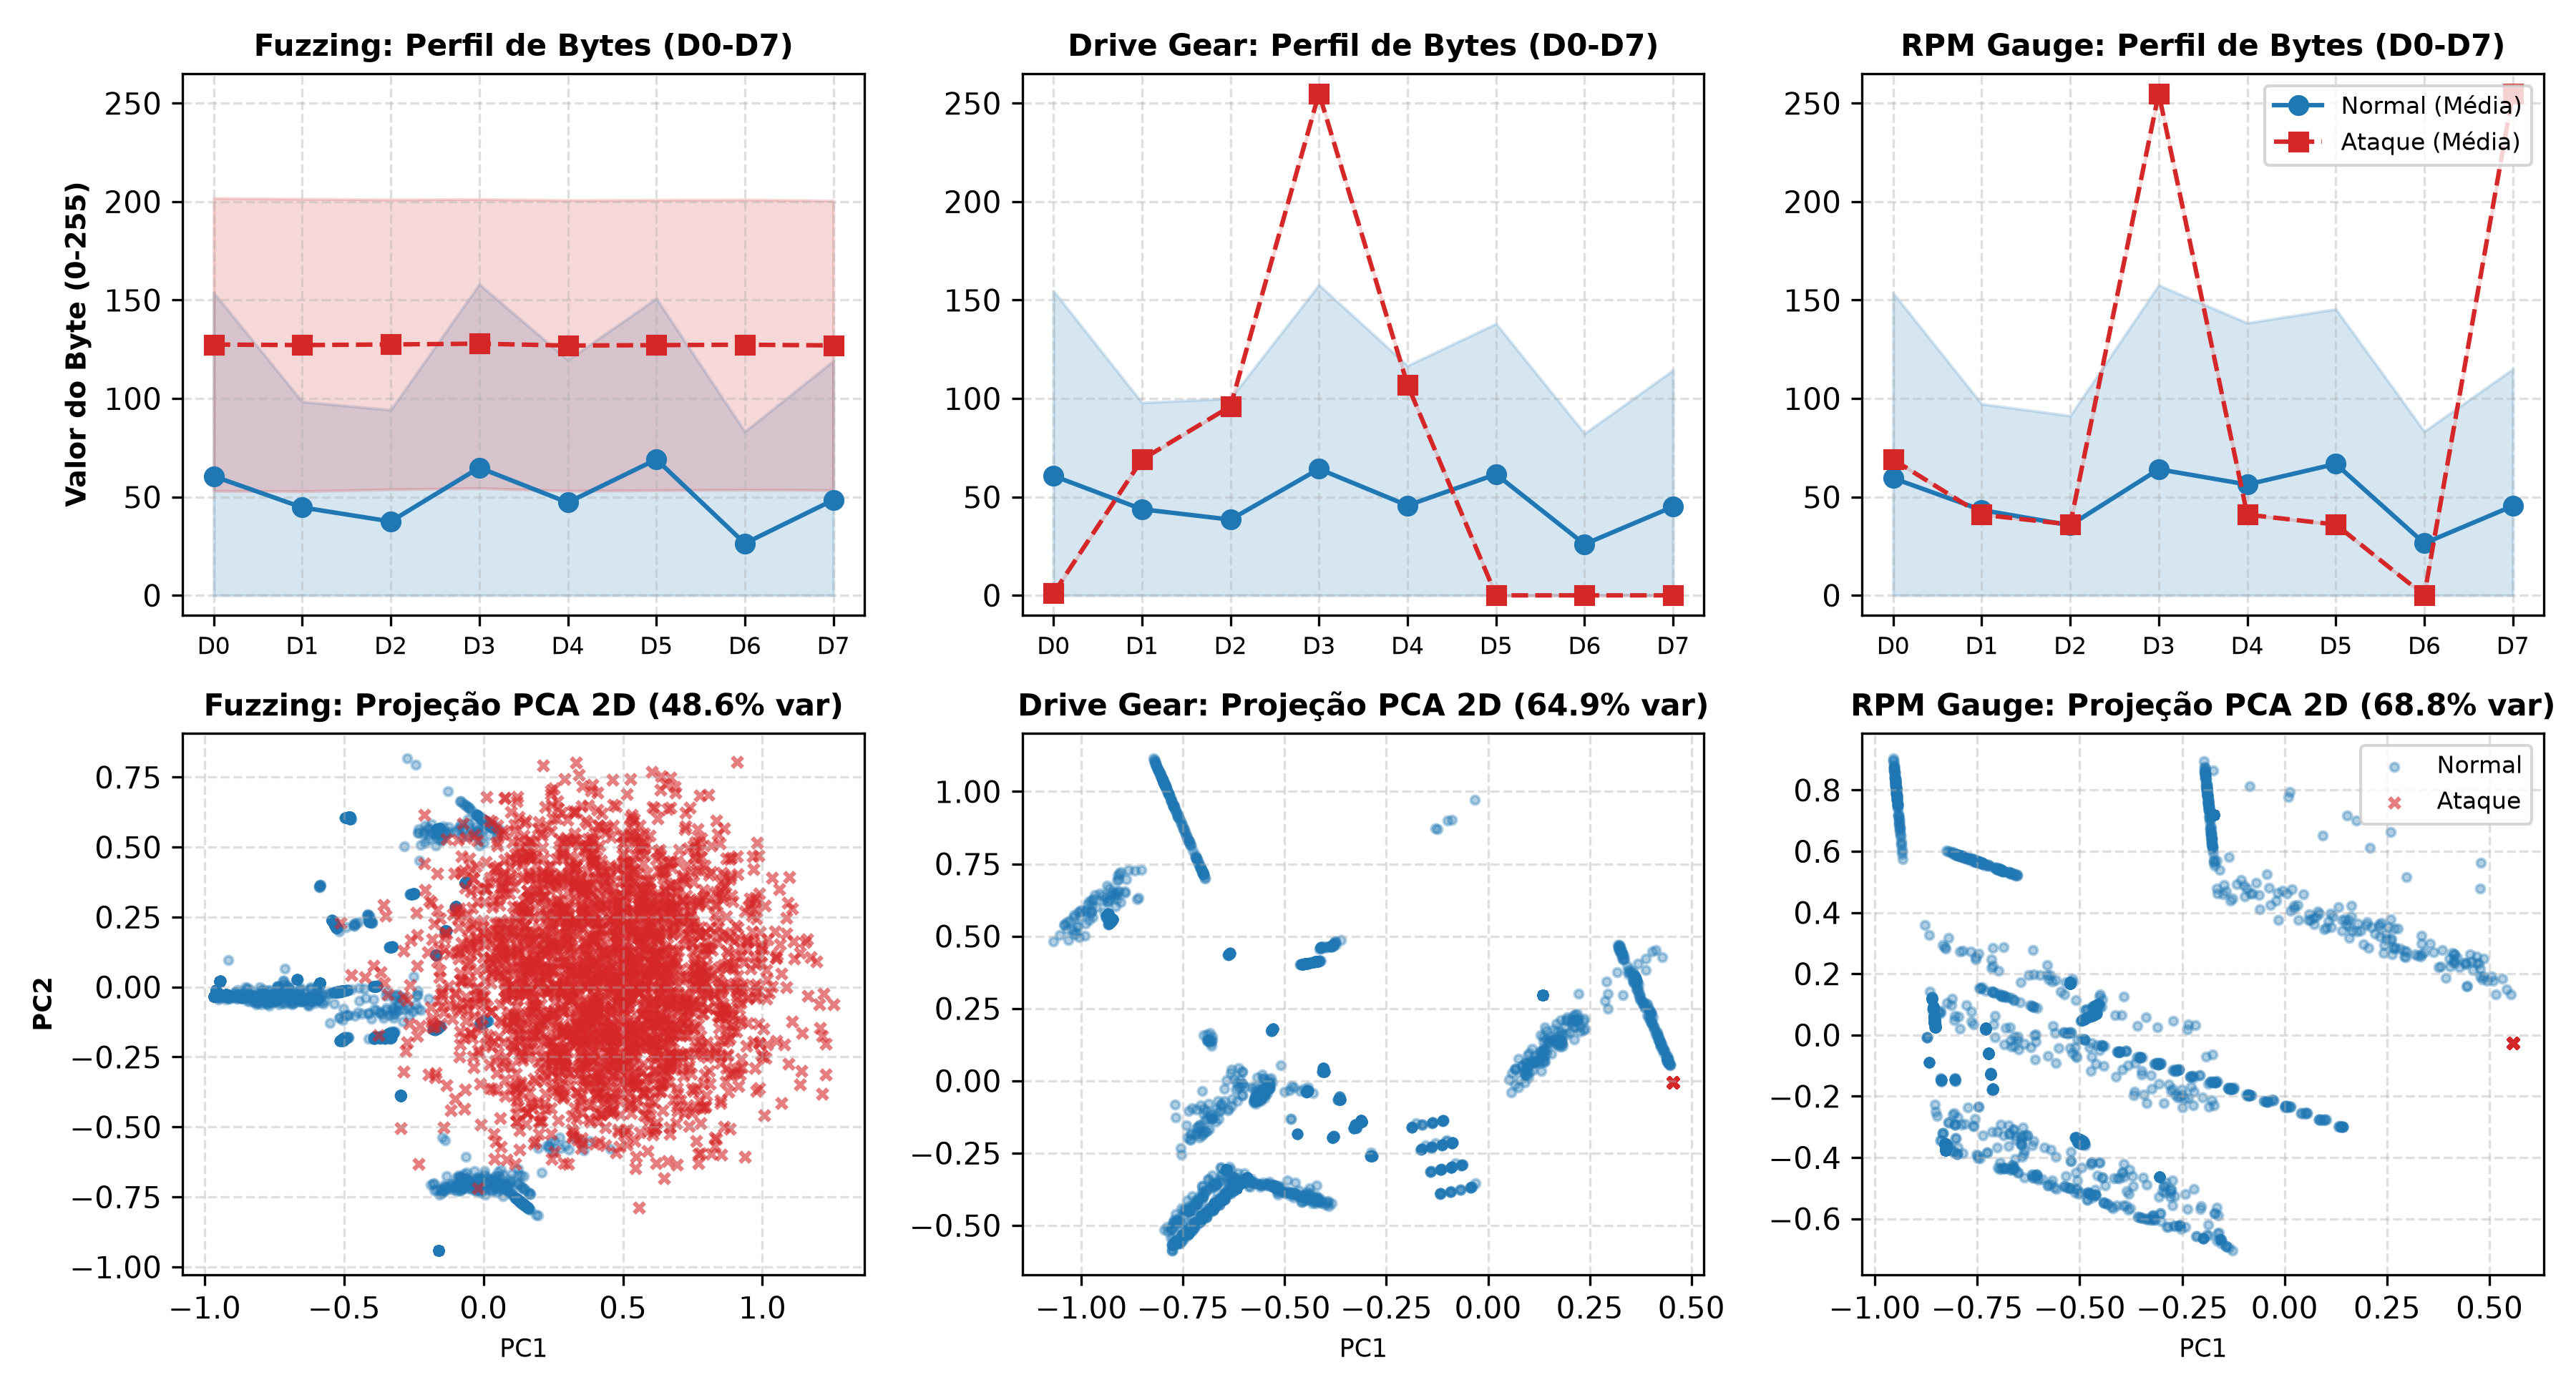
\includegraphics[width=0.95\textwidth]{fig_eda_signatures.png}
\caption{Análise Exploratória de Dados (EDA) sobre as partições de Treino e Validação: na linha superior, os perfis médios e faixas de desvio padrão dos bytes $D_0$ a $D_7$ para tráfego Normal (azul) versus Ataque (vermelho); na linha inferior, a projeção 2D via PCA dos payloads normalizados ($D_i / 255$), evidenciando a dispersão uniforme do Fuzzing e os atratores pontuais determinísticos dos ataques de Spoofing.}
\label{fig:eda_signatures}
\end{figure*}

A análise da Fig.~\ref{fig:eda_signatures} revela propriedades estruturais decisivas:
\begin{itemize}
    \item No \textbf{Fuzzing}, enquanto o tráfego legítimo apresenta médias baixas nos bytes finais ($D_6, D_7 \approx 18\text{--}25$) devido ao preenchimento com zeros (\textit{padding}) e contadores restritos, o tráfego de ataque possui média próxima a $127{,}5$ e alto desvio padrão em todos os 8 bytes, espalhando-se por todo o hiperespaço na projeção PCA;
    \item No \textbf{Drive Gear} e no \textbf{RPM Gauge}, como os quadros de ataque repetem um único vetor determinístico constante, a variância intra-ataque é nula ($\sigma = 0$), projetando todas as $25.000$ amostras maliciosas em um único ponto geométrico no plano PCA. Além disso, no \textit{Drive Gear}, os primeiros bytes ($D_0=\texttt{0x01}, D_1=\texttt{0x45}$) coincidem com valores individuais frequentemente observados em outros identificadores normais do veículo, tornando a anomalia discernível apenas quando analisada a combinação conjunta até o 5º byte ($D_4 = \texttt{0x6b}$).
\end{itemize}

\section{Sistema Proposto pelo Artigo de Referência}

\subsection{Arquitetura do IPS e Mecanismo de Descarte Ativo}
Diferentemente de um IDS passivo, o IPS proposto por Araujo-Filho \textit{et al.} \cite{araujo2021efficient} atua diretamente na camada física e de enlace do barramento CAN para impedir que um quadro malicioso seja validado pelas ECUs receptoras. O sistema é composto por três módulos de hardware de baixo custo:
\begin{enumerate}
    \item \textbf{Agente de Detecção (Raspberry Pi 4 Model B, 4 GB RAM):} Executa o modelo de aprendizado de máquina pré-treinado sobre os primeiros $N$ bytes de dados recebidos via interface serial periférica (SPI);
    \item \textbf{Controlador CAN (Microchip MCP2515):} Monitora o barramento bit a bit, realiza a desserialização dos bytes à medida que trafegam e comunica-se com a Raspberry Pi via sinais SPI (\texttt{CS}, \texttt{INT}, \texttt{MISO}, \texttt{MOSI} e \texttt{CLK});
    \item \textbf{Transceptor CAN (Microchip MCP2551):} Converte os níveis lógicos digitais em sinais diferenciais físicos (\texttt{CAN High} e \texttt{CAN Low}) e permite a transmissão de até 20 bits dominantes consecutivos.
\end{enumerate}

O protocolo CAN estipula que um quadro somente é considerado válido e entregue à camada de aplicação das ECUs receptoras se não ocorrer nenhum erro até o penúltimo bit (6º bit) do campo de Fim de Quadro (\textit{End of Frame} -- EOF) \cite{bosch1991can}. Ademais, a regra de preenchimento de bits (\textit{bit stuffing}) determina que, após 5 bits consecutivos de mesma polaridade, o transmissor deve inserir um bit de polaridade oposta. Caso qualquer nó detecte 6 bits consecutivos de mesma polaridade entre o início do quadro e o delimitador de CRC, todas as ECUs abortam imediatamente a recepção do quadro atual e entram em estado de erro. O IPS explora exatamente essa especificação: ao classificar os primeiros $N$ bytes como maliciosos, o Agente de Detecção comanda o transceptor para injetar uma sequência de 6 bits dominantes (`0`), gerando um \textit{Error Frame} que destrói o quadro malicioso ainda em trânsito.

\subsection{Restrição Física de Tempo Real ($T_{\text{DetectionMax}}$)}
Um quadro CAN 2.0A padrão com $D = 8$ bytes de dados possui a seguinte estrutura sequencial: \textit{Start of Frame} (SOF, 1 bit), Campo de Arbitragem (12 bits), Campo de Controle (6 bits), Campo de Dados ($8 \times 8 = 64$ bits), Campo de CRC (16 bits), Campo de ACK (2 bits) e Fim de Quadro (EOF, 7 bits), totalizando 108 bits (desconsiderando bits de \textit{stuffing}).

Como a detecção inicia imediatamente após a recepção do $N$-ésimo byte de dados e a destruição do quadro requer que o primeiro bit do \textit{Error Frame} seja transmitido antes do 6º bit do EOF, o número de bits restantes na transmissão após o $N$-ésimo byte é dado por $8 \cdot (8 - N)$ bits de dados remanescentes somados a $16 \text{ (CRC)} + 2 \text{ (ACK)} + 1 \text{ (primeiro bit do EOF)} = 19$ bits. Portanto, o tempo máximo disponível para o algoritmo classificar o quadro ($T_{\text{DetectionMax}}$) é regido pela Equação~\eqref{eq:tdetmax}:
\begin{equation}
T_{\text{DetectionMax}} = \left[19 + 8 \cdot (8 - N)\right] \cdot T_{\text{bit}} - T_{\text{Delay}},
\label{eq:tdetmax}
\end{equation}
onde $T_{\text{bit}}$ é a duração de um bit no barramento e $T_{\text{Delay}}$ representa os atrasos elétricos de propagação entre transceptor, controlador e processador. Em redes CAN automotivas de alta velocidade ($500\,\text{kbps}$), tem-se $T_{\text{bit}} = 2\,\mu\text{s}$. Para $N = 5$ bytes de dados, restam $[19 + 8 \cdot (8 - 5)] = 43$ bits, o que impõe o limite estrito:
\begin{equation}
T_{\text{DetectionMax}}(N=5) = 43 \cdot T_{\text{bit}} - T_{\text{Delay}} \le 86\,\mu\text{s}.
\label{eq:limit86}
\end{equation}
Conforme demonstrado no artigo original, utilizar $N > 5$ bytes reduz a janela para $T_{\text{DetectionMax}}(N=6) = 35 \cdot T_{\text{bit}} = 70\,\mu\text{s}$, valor insuficiente para acomodar o tempo de inferência na Raspberry Pi 4 ($\sim 78\text{--}79\,\mu\text{s}$). Assim, a redução do número de bytes inspecionados para $N \le 5$ é condição física indispensável para a viabilidade do IPS.

\subsection{Algoritmos de Detecção Não Supervisionados}
Para evitar que o modelo dependa do identificador da mensagem (permitindo generalização e operação direta sobre o fluxo de dados), o vetor de entrada de um modelo de $N$ bytes consiste exclusivamente nos primeiros $N$ bytes de dados normalizados no intervalo $[0, 1]$:
\begin{equation}
\mathbf{x}_N = \left[ \frac{D_0}{255}, \frac{D_1}{255}, \dots, \frac{D_{N-1}}{255} \right] \in [0, 1]^N.
\label{eq:normalization}
\end{equation}
O artigo avalia duas famílias de algoritmos treinadas unicamente com amostras normais ($\mathbf{x}_N^{(i)} \in \mathcal{D}_{\text{normal}}$):
\begin{itemize}
    \item \textbf{One-Class SVM (OCSVM) \cite{scholkopf2001estimating}:} Mapeia os dados normais para um espaço de características de alta dimensão por meio de uma função de kernel (sendo escolhido o kernel de Base Radial -- RBF, $K(\mathbf{x}, \mathbf{x}') = \exp(-\gamma \|\mathbf{x} - \mathbf{x}'\|^2)$) e encontra um hiperplano de margem máxima que separa a imagem dos dados normais da origem, controlado pela fração máxima de \textit{outliers} $\nu \in (0, 1]$;
    \item \textbf{Isolation Forest (iForest) \cite{liu2008isolation}:} Constrói um conjunto (\textit{ensemble}) de $T$ árvores binárias de isolamento (\textit{iTrees}) sobre subamostras de tamanho $\psi$ (\texttt{max\_samples}). Em cada nó interno, seleciona-se aleatoriamente um atributo $q \in \{0, \dots, N-1\}$ e um ponto de corte $p$ entre o mínimo e o máximo daquele atributo na subamostra. Como anomalias situam-se em regiões esparsas, elas são isoladas próximas à raiz (menor comprimento médio de caminho $E[h(\mathbf{x})]$), produzindo um escore de anomalia $s(\mathbf{x}, \psi) = 2^{-E[h(\mathbf{x})]/c(\psi)}$.
\end{itemize}
Combinando as duas famílias com $N \in \{1, \dots, 8\}$ bytes, definem-se os 16 modelos avaliados: $\text{OCSVM\_1F}$ a $\text{OCSVM\_8F}$ e $\text{iForest\_1F}$ a $\text{iForest\_8F}$.

\section{Otimizações Computacionais e Calibração Propostas na Replicação}

Durante a implementação e execução da replicação em larga escala (12,9 milhões de mensagens totais), identificamos desafios computacionais e de aprendizado estatístico não detalhados explicitamente no texto original, para os quais implementamos três melhorias metodológicas no código-fonte:

\subsection{Indexação em Streaming e Blindagem de Partições}
Os três arquivos CSV brutos somam mais de 12,9 milhões de registros e apresentam linhas com comprimentos variáveis quando o campo \textit{Data Length Code} ($\text{DLC} < 8$) omite bytes finais. Implementamos em \texttt{utils.py} um parser vetorizado em duas fases que varre a contagem exata de classes via \textit{streaming} e persiste os índices de partição em arquivos binários compactados (\texttt{.npz}). Isso garante que a seleção das $250.000$ amostras normais de treino/validação e $25.000$ de ataque ocorra com semente fixa ($\text{seed}=42$), mantendo os milhões de quadros de teste 100\% isolados em disco até o momento da avaliação final.

\subsection{Fatoração Exata do Limiar na Validação Cruzada do iForest}
No \textit{Isolation Forest}, a estrutura topológica das árvores construídas em cada \textit{fold} depende exclusivamente do número de estimadores (\texttt{n\_estimators}) e do tamanho da subamostra (\texttt{max\_samples}), enquanto o hiperparâmetro \texttt{contamination} ($c$) atua apenas no pós-processamento para definir o limiar de corte ($\text{offset} = \text{percentil}_{100 \cdot c}(s_{\text{treino}})$). Em \texttt{run\_experiments.py}, implementamos um mecanismo de cache de escores por \textit{fold} que ajusta as árvores uma única vez para cada par $(\texttt{n\_estimators}, \texttt{max\_samples})$ e avalia instantaneamente múltiplos valores de \texttt{contamination} em memória, reduzindo o tempo de busca em grade em $4\times$ com equivalência numérica exata bit a bit.

\subsection{Profundidade de Subamostragem (\texttt{max\_samples}) em Ataques de Spoofing}
Na implementação padrão da biblioteca \texttt{scikit-learn}, o parâmetro \texttt{max\_samples="auto"} limita cada árvore a apenas $\psi = 256$ amostras e profundidade máxima $\lceil \log_2(256) \rceil = 8$ níveis. Embora árvores rasas ($\psi \in \{256, 512\}$) isolem perfeitamente ruídos aleatórios de \textit{Fuzzing}, verificamos experimentalmente que elas sofrem degradação severa nos ataques de \textit{Drive Gear} e \textit{RPM Gauge Spoofing}.

A explicação matemática reside na natureza multimodal do barramento CAN: o conjunto de treinamento possui $225.000$ quadros normais distribuídos entre cerca de 40 a 80 identificadores distintos. Uma subamostra de $\psi = 256$ quadros captura apenas $0{,}11\%$ do conjunto de treino (cerca de 3 a 5 exemplos por ID). Nos ataques de \textit{Spoofing}, cada byte individual do payload forjado ($\text{ex.: } D_0=\texttt{0x01}, D_1=\texttt{0x45}$) ocorre legitimamente em outros IDs normais; apenas a combinação conjunta dos 5 bytes ($[D_0, \dots, D_4]$) é anômala. Com limite de profundidade igual a 8 ou 9 cortes aleatórios divididos entre 5 atributos, as árvores atingem a profundidade máxima antes de isolar a combinação conjunta de 5 bytes, estacionando o escore do quadro de \textit{Spoofing} apenas no percentil $3{,}4\%\text{--}5{,}8\%$ da distribuição normal. Ao expandir a subamostragem para $\psi = 16.384$ ($\log_2(\psi) = 14$ níveis de profundidade), as árvores passam a particionar conjuntamente os 5 bytes, reduzindo a taxa de falsos positivos necessária para $100\%$ de \textit{Recall} de $3{,}42\%$ para $1{,}11\%$ no \textit{Drive Gear} e de $5{,}82\%$ para $0{,}48\%$ no \textit{RPM Gauge}.

\section{Metodologia}

\subsection{Dados Utilizados pelo Artigo de Referência}
Os experimentos do artigo de referência foram conduzidos sobre três conjuntos de dados públicos do \textit{Car-Hacking Dataset} \cite{seo2018gids}: \textit{Fuzzing}, \textit{Drive Gear Spoofing} e \textit{RPM Gauge Spoofing}. Cada registro contém o carimbo de tempo (\textit{Timestamp}), o identificador hexadecimal (\textit{CAN ID}), o tamanho da carga útil (\textit{DLC}, de 0 a 8), os bytes de dados $D_0 \dots D_7$ e o rótulo de classe (\texttt{R} para mensagem normal e \texttt{T} para mensagem injetada/maliciosa). A Tabela~\ref{tab:dataset_audit} apresenta a auditoria exata da composição de cada dataset, que coincide integralmente com a Tabela 2 do artigo original.

\begin{table}[htbp]
\caption{Volume Total e Proporção de Classes nos Três Conjuntos de Dados (Reprodução da Tabela 2 do Artigo)}
\label{tab:dataset_audit}
\centering
\scriptsize
\setlength{\tabcolsep}{3.5pt}
\begin{tabular}{lrrrr}
\toprule
\textbf{Dataset} & \textbf{Total} & \textbf{Normais} & \textbf{Ataques} & \textbf{\% Ataque} \\
\midrule
Fuzzing & 3.838.860 & 3.347.013 & 491.847 & 12,81\% \\
Drive Gear & 4.443.142 & 3.845.890 & 597.252 & 13,44\% \\
RPM Gauge & 4.621.702 & 3.966.805 & 654.897 & 14,17\% \\
\bottomrule
\end{tabular}
\end{table}

Seguindo o protocolo da Seção V-A do artigo original (Tabelas 3, 4 e 5 do artigo), o \textit{pipeline} implementado em \texttt{utils.py} padroniza a entrada retendo exclusivamente os quadros completos de $\text{DLC}=8$ ($12$ colunas no CSV), excluindo $87.836$ ($2{,}29\%$), $40.165$ ($0{,}90\%$) e $41.476$ ($0{,}90\%$) mensagens normais com carga útil incompleta ($\text{DLC} < 8$) em \textit{Fuzzing}, \textit{Drive Gear} e \textit{RPM Gauge}, respectivamente. Todos os quadros de ataque possuem $\text{DLC}=8$. As partições resultantes (resumidas na Tabela~\ref{tab:splits}) obedecem a três etapas:
\begin{enumerate}
    \item Selecionam-se aleatoriamente $250.000$ mensagens normais e $25.000$ mensagens de ataque ($\text{DLC}=8$) para o processo de treinamento e validação cruzada de 10 \textit{folds};
    \item As $250.000$ mensagens normais são divididas em 10 blocos disjuntos de $25.000$ mensagens. Em cada uma das 10 iterações da validação cruzada, 9 blocos ($225.000$ mensagens exclusivamente normais) formam o conjunto de \textbf{Treinamento}, enquanto o bloco restante ($25.000$ normais) é combinado às $25.000$ mensagens de ataque para formar um conjunto de \textbf{Validação} balanceado ($50.000$ amostras, 50\% normal e 50\% ataque), utilizado para seleção de hiperparâmetros;
    \item Todas as mensagens normais ($\text{DLC}=8$) e de ataque remanescentes compõem o conjunto de \textbf{Teste} final ($3.476.024$, $4.127.977$ e $4.305.226$ mensagens, mantendo a proporção natural desbalanceada de $\sim 86\%$ normal e $\sim 14\%$ ataque).
\end{enumerate}

\begin{table}[htbp]
\caption{Formação dos Conjuntos de Treinamento, Validação (por Fold) e Teste ($\text{DLC}=8$; Baseado nas Tabelas 3, 4 e 5 do Artigo)}
\label{tab:splits}
\centering
\scriptsize
\setlength{\tabcolsep}{4pt}
\begin{tabular}{llrrr}
\toprule
\textbf{Dataset} & \textbf{Conjunto} & \textbf{Normais} & \textbf{Ataques} & \textbf{Total} \\
\midrule
\multirow{3}{*}{Fuzzing} & Treinamento (9 folds) & 225.000 & 0 & 225.000 \\
 & Validação (1 fold) & 25.000 & 25.000 & 50.000 \\
 & Teste Final & 3.009.177 & 466.847 & 3.476.024 \\
\midrule
\multirow{3}{*}{Drive Gear} & Treinamento (9 folds) & 225.000 & 0 & 225.000 \\
 & Validação (1 fold) & 25.000 & 25.000 & 50.000 \\
 & Teste Final & 3.555.725 & 572.252 & 4.127.977 \\
\midrule
\multirow{3}{*}{RPM Gauge} & Treinamento (9 folds) & 225.000 & 0 & 225.000 \\
 & Validação (1 fold) & 25.000 & 25.000 & 50.000 \\
 & Teste Final & 3.675.329 & 629.897 & 4.305.226 \\
\bottomrule
\end{tabular}
\end{table}

\subsection{Métricas de Avaliação e Testes Estatísticos}
A eficácia de classificação no conjunto de teste é mensurada por quatro métricas derivadas das contagens de Verdadeiros Positivos ($TP$, ataques corretamente detectados), Falsos Positivos ($FP$, quadros normais classificados como ataque), Verdadeiros Negativos ($TN$) e Falsos Negativos ($FN$):
\begin{align}
\text{Acurácia} &= \frac{TP + TN}{TP + TN + FP + FN}, \label{eq:acc} \\
\text{Precisão} &= \frac{TP}{TP + FP}, \quad \text{Recall} = \frac{TP}{TP + FN}, \label{eq:prec_rec} \\
\text{F1-Score} &= 2 \cdot \frac{\text{Precisão} \cdot \text{Recall}}{\text{Precisão} + \text{Recall}}. \label{eq:f1}
\end{align}

Para avaliar a escolha do menor número de bytes $N$ frente ao modelo completo de 8 bytes, aplicou-se inicialmente a sequência de três testes descrita na Seção VI-B do artigo ($\alpha = 0{,}05$), complementada por um teste formal de equivalência pareado:
\begin{enumerate}
    \item \textbf{Teste de D'Agostino-Pearson:} Verifica se as taxas de acurácia nos 10 \textit{folds} de cada modelo são compatíveis com normalidade ($p > 0{,}05$);
    \item \textbf{One-Way ANOVA:} Avalia a hipótese nula de igualdade entre as médias globais dos 16 modelos;
    \item \textbf{Teste Post-Hoc de Tukey HSD (\textit{Honestly Significant Difference}):} Compara os modelos par a par contra $\text{iForest\_8F}$ entre os candidatos com acurácia média $\ge 85\%$, identificando o menor $N$ para o qual $p > 0{,}05$ (ausência de diferença estatisticamente significativa detectada);
    \item \textbf{Teste Pareado de Equivalência TOST (\textit{Two One-Sided Tests}):} Como não rejeitar a hipótese nula no teste de Tukey não prova equivalência formal, aplicamos em \texttt{post\_analysis.py} o teste TOST pareado por \textit{fold} contra $\text{iForest\_8F}$ com margem de equivalência $\Delta = \pm 1{,}00\%$ p.p. ($\alpha = 0{,}05$). Ressalta-se, como limitação inerente ao protocolo 10-\textit{fold} adotado, que os \textit{folds} compartilham $9/10$ dos dados normais de treinamento (e, no \textit{Car-Hacking}, as mesmas $25.000$ amostras de ataque na validação), de modo que os valores-$p$ nominais devem ser interpretados sob essa dependência estrutural.
\end{enumerate}

\subsection{Segundo Conjunto de Dados Escolhido: Prototype Speedometer Spoofing}
Para avaliar a capacidade de generalização do sistema proposto fora do conjunto \textit{Car-Hacking}, selecionou-se um segundo conjunto de dados público de intrusão CAN (repositório \textit{4TU.ResearchData} \cite{fourtu_can_dataset}) capturado com a ferramenta \texttt{candump} em uma bancada física real (\textit{Prototype}), composta por um painel de instrumentos Volkswagen, duas ECUs baseadas em Arduino com \textit{CAN bus shields} e um \textit{joystick} que simula o acelerador em condução urbana. Entre os cenários disponíveis no repositório, optou-se pelo arquivo \texttt{spoofing\_speedometer.log} por dois critérios metodológicos: (i) trata-se de um ataque físico real injetado por uma ECU comprometida sem substituir o tráfego legítimo por inundação bruta (diferentemente do cenário de DoS por \textit{flooding}, que altera drasticamente o volume da rede); e (ii) apresenta volume suficiente de quadros maliciosos ($5.772$ pacotes de ataque entre as linhas $53.966$ e $76.682$, em um total de $146.109$ pacotes, sendo $145.546$ com $\text{DLC}=8$) para sustentar uma validação cruzada de 10 \textit{folds} e um conjunto de teste blindado.

A Análise Exploratória de Dados (EDA) foi conduzida estritamente sobre a partição de Treino e Validação ($27.500$ quadros: $25.000$ normais e $2.500$ ataques), mantendo os $118.046$ quadros de teste completamente isolados. Observou-se que:
\begin{itemize}
    \item O tráfego normal de 8 bytes distribui-se por 14 \textit{CAN IDs}, dos quais o identificador do velocímetro (\texttt{0x05A0}) representa $6{,}31\%$ ($1.578/25.000$ quadros) e opera com payload normal $\mathbf{d}_{\text{norm}} = [\texttt{01, 80}, D_2, \texttt{00, 00, 00, 00, 00}]$, onde $D_2 \in [0, 28]$ ($\texttt{0x00}$ a $\texttt{0x1C}$, média $4{,}81 \pm 7{,}92$);
    \item Durante o ataque, a ECU comprometida força o ponteiro para $220\,\text{km/h}$ injetando $\mathbf{d}_{\text{atk}} = [\texttt{01, 80, 7e, 00, 00, 00, 00, 00}]$ no mesmo ID \texttt{0x05A0};
    \item Como consequência, os primeiros dois bytes ($D_0=\texttt{0x01}, D_1=\texttt{0x80}$) colidem em $6{,}31\%$ do tráfego normal (sendo indistinguíveis para $N=1$ e $N=2$), mas a partir do 3º byte ($D_2=\texttt{0x7E}=126$) a taxa de colisão cai para exatos $0{,}00\%$.
\end{itemize}

Devido à menor escala absoluta desse dataset em comparação ao \textit{Car-Hacking}, adaptou-se proporcionalmente o tamanho dos \textit{folds} preservando integralmente o protocolo de 10-\textit{Fold CV} sem vazamento de dados (Tabela~\ref{tab:splits_spd}): cada iteração treina com $22.500$ quadros normais (9 \textit{folds} de $2.500$) e valida com $500$ quadros balanceados ($250$ normais + $250$ ataques), reservando $118.046$ quadros ($114.774$ normais + $3.272$ ataques) para o teste final.

\begin{table}[htbp]
\caption{Particionamento Proporcional (10-Fold CV) para o Dataset Speedometer Spoofing}
\label{tab:splits_spd}
\centering
\scriptsize
\setlength{\tabcolsep}{4pt}
\begin{tabular}{lrrr}
\toprule
\textbf{Conjunto (DLC = 8)} & \textbf{Normais} & \textbf{Ataques} & \textbf{Total} \\
\midrule
Treinamento por Fold (9 folds) & 22.500 & 0 & 22.500 \\
Validação por Fold (balanceada) & 250 & 250 & 500 \\
Pool Exclusivo da EDA (Train+Val) & 25.000 & 2.500 & 27.500 \\
Teste Final (Blindado) & 114.774 & 3.272 & 118.046 \\
\bottomrule
\end{tabular}
\end{table}

\section{Resultados e Discussões}

\subsection{Desempenho por Número de Bytes no Ataque Fuzzing (Tabela 7 e Figura 5)}
Seguindo o critério estabelecido na Seção VI-A do artigo original, modelos com acurácia inferior a 85\% são desconsiderados para aplicação prática no IPS. A Tabela~\ref{tab:table7_fuzzing} confronta lado a lado os resultados reportados na Tabela 7 do artigo original com os resultados obtidos em nossa replicação sobre os $3.476.024$ quadros de teste do dataset \textit{Fuzzing}.

\begin{table}[htbp]
\caption{Desempenho de Detecção no Ataque Fuzzing: Artigo Original vs. Nossa Replicação (Tabela 7 do Artigo)}
\label{tab:table7_fuzzing}
\centering
\scriptsize
\setlength{\tabcolsep}{2.8pt}
\begin{tabular}{lccccccc}
\toprule
\multirow{2}{*}{\textbf{Modelo}} & \multicolumn{2}{c}{\textbf{Acurácia (\%)}} & \multicolumn{2}{c}{\textbf{Precisão (\%)}} & \multicolumn{2}{c}{\textbf{Recall (\%)}} & \textbf{F1 (\%)} \\
\cmidrule(lr){2-3} \cmidrule(lr){4-5} \cmidrule(lr){6-7} \cmidrule(lr){8-8}
 & \textbf{Artigo} & \textbf{Replic.} & \textbf{Artigo} & \textbf{Replic.} & \textbf{Artigo} & \textbf{Replic.} & \textbf{Replic.} \\
\midrule
iForest\_8F & 99,72 & \textbf{99,55} & 98,00 & \textbf{97,03} & 99,97 & \textbf{99,73} & 98,36 \\
iForest\_7F & 99,59 & \textbf{99,49} & 97,07 & \textbf{96,88} & 99,97 & \textbf{99,38} & 98,11 \\
iForest\_6F & 99,31 & \textbf{98,72} & 95,20 & \textbf{91,56} & 99,94 & \textbf{99,69} & 95,45 \\
iForest\_5F & 99,31 & \textbf{98,70} & 95,22 & \textbf{91,66} & 99,90 & \textbf{99,35} & 95,35 \\
iForest\_4F & 99,14 & \textbf{97,90} & 94,24 & \textbf{88,44} & 99,73 & \textbf{97,03} & 92,54 \\
iForest\_3F & 98,57 & \textbf{97,96} & 90,66 & \textbf{88,70} & 99,62 & \textbf{97,20} & 92,76 \\
iForest\_2F & 95,77 & \textbf{95,88} & 77,08 & \textbf{86,45} & 98,66 & \textbf{82,17} & 84,26 \\
iForest\_1F & $<85$* & \textbf{62,41}* & --- & 25,98 & --- & 97,27 & 41,01 \\
\midrule
OCSVM\_8F & 97,06 & \textbf{90,62} & 83,05 & \textbf{60,36} & 99,92 & \textbf{87,90} & 71,57 \\
OCSVM\_7F & 96,59 & \textbf{96,46} & 81,15 & \textbf{85,82} & 99,78 & \textbf{88,23} & 87,01 \\
OCSVM\_6F & 95,67 & \textbf{96,58} & 79,01 & \textbf{92,45} & 97,63 & \textbf{81,18} & 86,45 \\
OCSVM\_5F & 86,74 & \textbf{85,63} & 52,32 & \textbf{47,84} & 91,66 & \textbf{77,27} & 59,10 \\
OCSVM\_4F & $<85$* & \textbf{75,29}* & --- & 31,10 & --- & 69,10 & 42,89 \\
OCSVM\_3F & $<85$* & \textbf{68,51}* & --- & 23,60 & --- & 60,10 & 33,89 \\
OCSVM\_2F & $<85$* & \textbf{69,35}* & --- & 20,37 & --- & 44,08 & 27,86 \\
OCSVM\_1F & $<85$* & \textbf{59,92}* & --- & 14,21 & --- & 39,38 & 20,88 \\
\bottomrule
\multicolumn{8}{l}{\tiny *Modelos com acurácia $< 85\%$ foram desconsiderados no artigo original e na replicação.}
\end{tabular}
\end{table}

Os resultados da Tabela~\ref{tab:table7_fuzzing} e a curva de progressão exibida na Fig.~\ref{fig:bytes_progression} demonstram uma concordância notável entre a nossa replicação e o artigo de referência:
\begin{enumerate}
    \item \textbf{Reprodução exata do limiar de descarte ($<85\%$):} Tanto no artigo original quanto em nossa replicação, exatamente os mesmos cinco modelos ($\text{iForest\_1F}$ e $\text{OCSVM\_1F}\dots\text{4F}$) ficaram abaixo do corte de 85\% de acurácia. Fisicamente, um único byte ($2^8 = 256$ estados possíveis) não detém entropia suficiente para discriminar o tráfego legítimo de um veículo (cujos sensores, contadores e \textit{checksums} percorrem quase todos os valores de \texttt{0x00} a \texttt{0xFF} em $D_0$) de uma injeção de \textit{Fuzzing};
    \item \textbf{Crescimento monotônico e saturação a partir de $N=5$:} À medida que o número de bytes $N$ aumenta, a variedade normal passa a ocupar uma fração exponencialmente menor do espaço de estados ($256^N$). A acurácia do iForest cresce de $62{,}41\%$ ($1\text{F}$) para $95{,}88\%$ ($2\text{F}$), $97{,}96\%$ ($3\text{F}$), $98{,}70\%$ ($5\text{F}$) e $99{,}55\%$ ($8\text{F}$), ficando a apenas $0{,}17\%$ do topo reportado no artigo ($99{,}72\%$);
    \item \textbf{Superioridade do iForest sobre o OCSVM:} Embora os modelos $\text{OCSVM\_5F}$ ($85{,}63\%$ vs. $86{,}74\%$), $\text{OCSVM\_6F}$ ($96{,}58\%$ vs. $95{,}67\%$) e $\text{OCSVM\_7F}$ ($96{,}46\%$ vs. $96{,}59\%$) tenham replicado fielmente os valores do artigo, o algoritmo iForest supera consistentemente o OCSVM em precisão e recall com menos bytes de entrada.
\end{enumerate}

\begin{figure}[htbp]
\centering
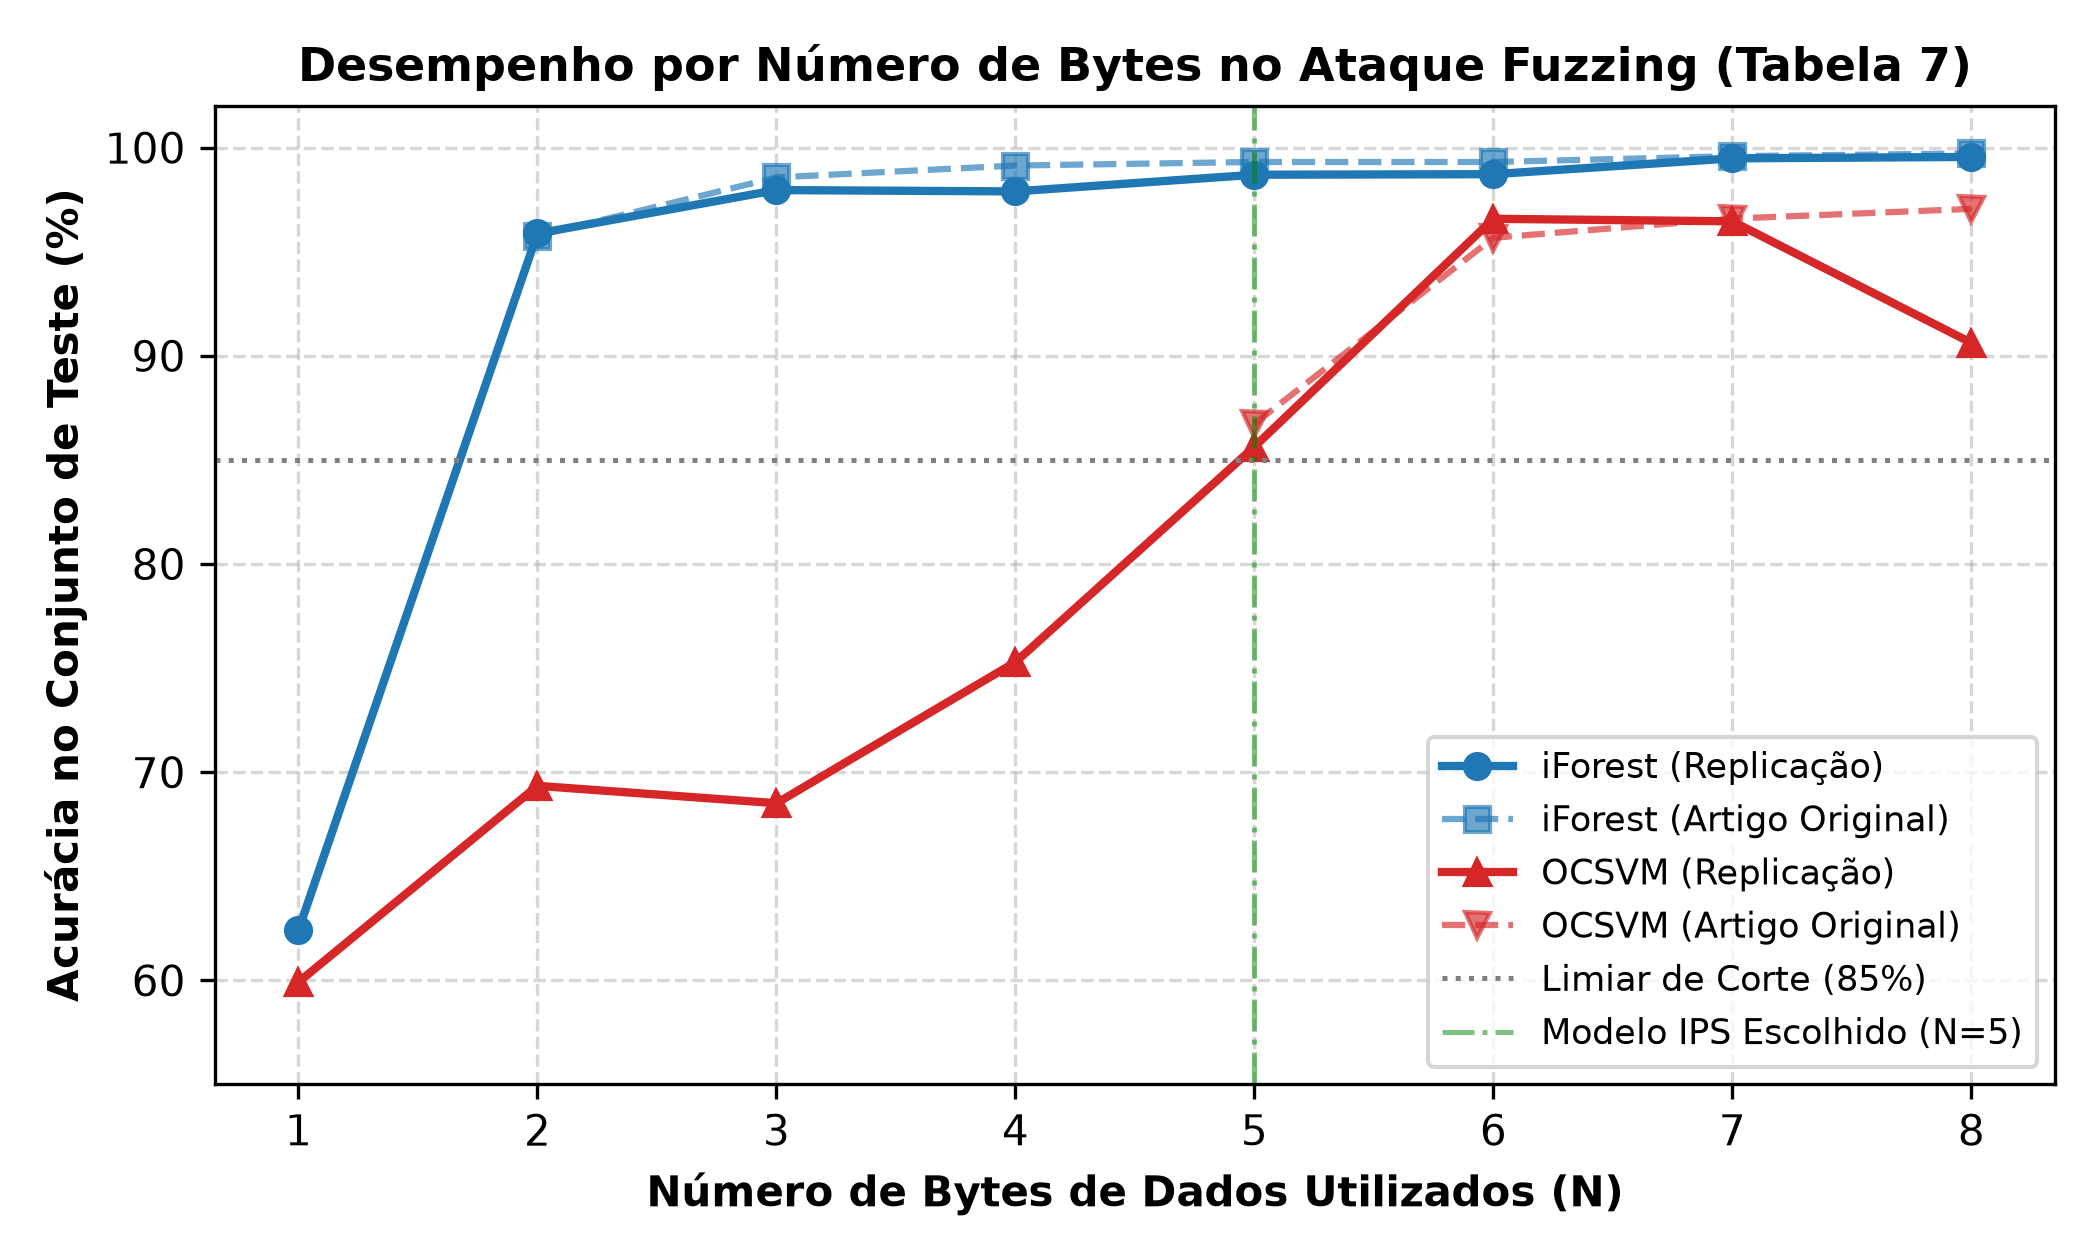
\includegraphics[width=0.98\columnwidth]{fig_bytes_progression.png}
\caption{Evolução da acurácia no conjunto de teste em função do número de bytes de dados ($N = 1 \dots 8$) para o ataque Fuzzing, comparando os resultados da nossa replicação (linhas contínuas) com os reportados no artigo original (linhas tracejadas).}
\label{fig:bytes_progression}
\end{figure}

A Fig.~\ref{fig:fig5_cm} reproduz as matrizes de confusão da Figura 5 do artigo para os modelos de 5 a 8 bytes. Observa-se que os modelos $\text{iForest\_8F}$ e $\text{iForest\_7F}$ atingem taxas de falsos positivos (FP) de apenas $0{,}47\%$ e $0{,}50\%$ (contra $0{,}32\%$ e $0{,}47\%$ no artigo original) e taxas de verdadeiros positivos (TP) de $99{,}73\%$ e $99{,}38\%$, enquanto os modelos $\text{iForest\_6F}$ e $\text{iForest\_5F}$ mantêm falsos positivos em $1{,}43\%$ e $1{,}40\%$ com detecção superior a $99{,}35\%$.

\begin{figure}[htbp]
\centering
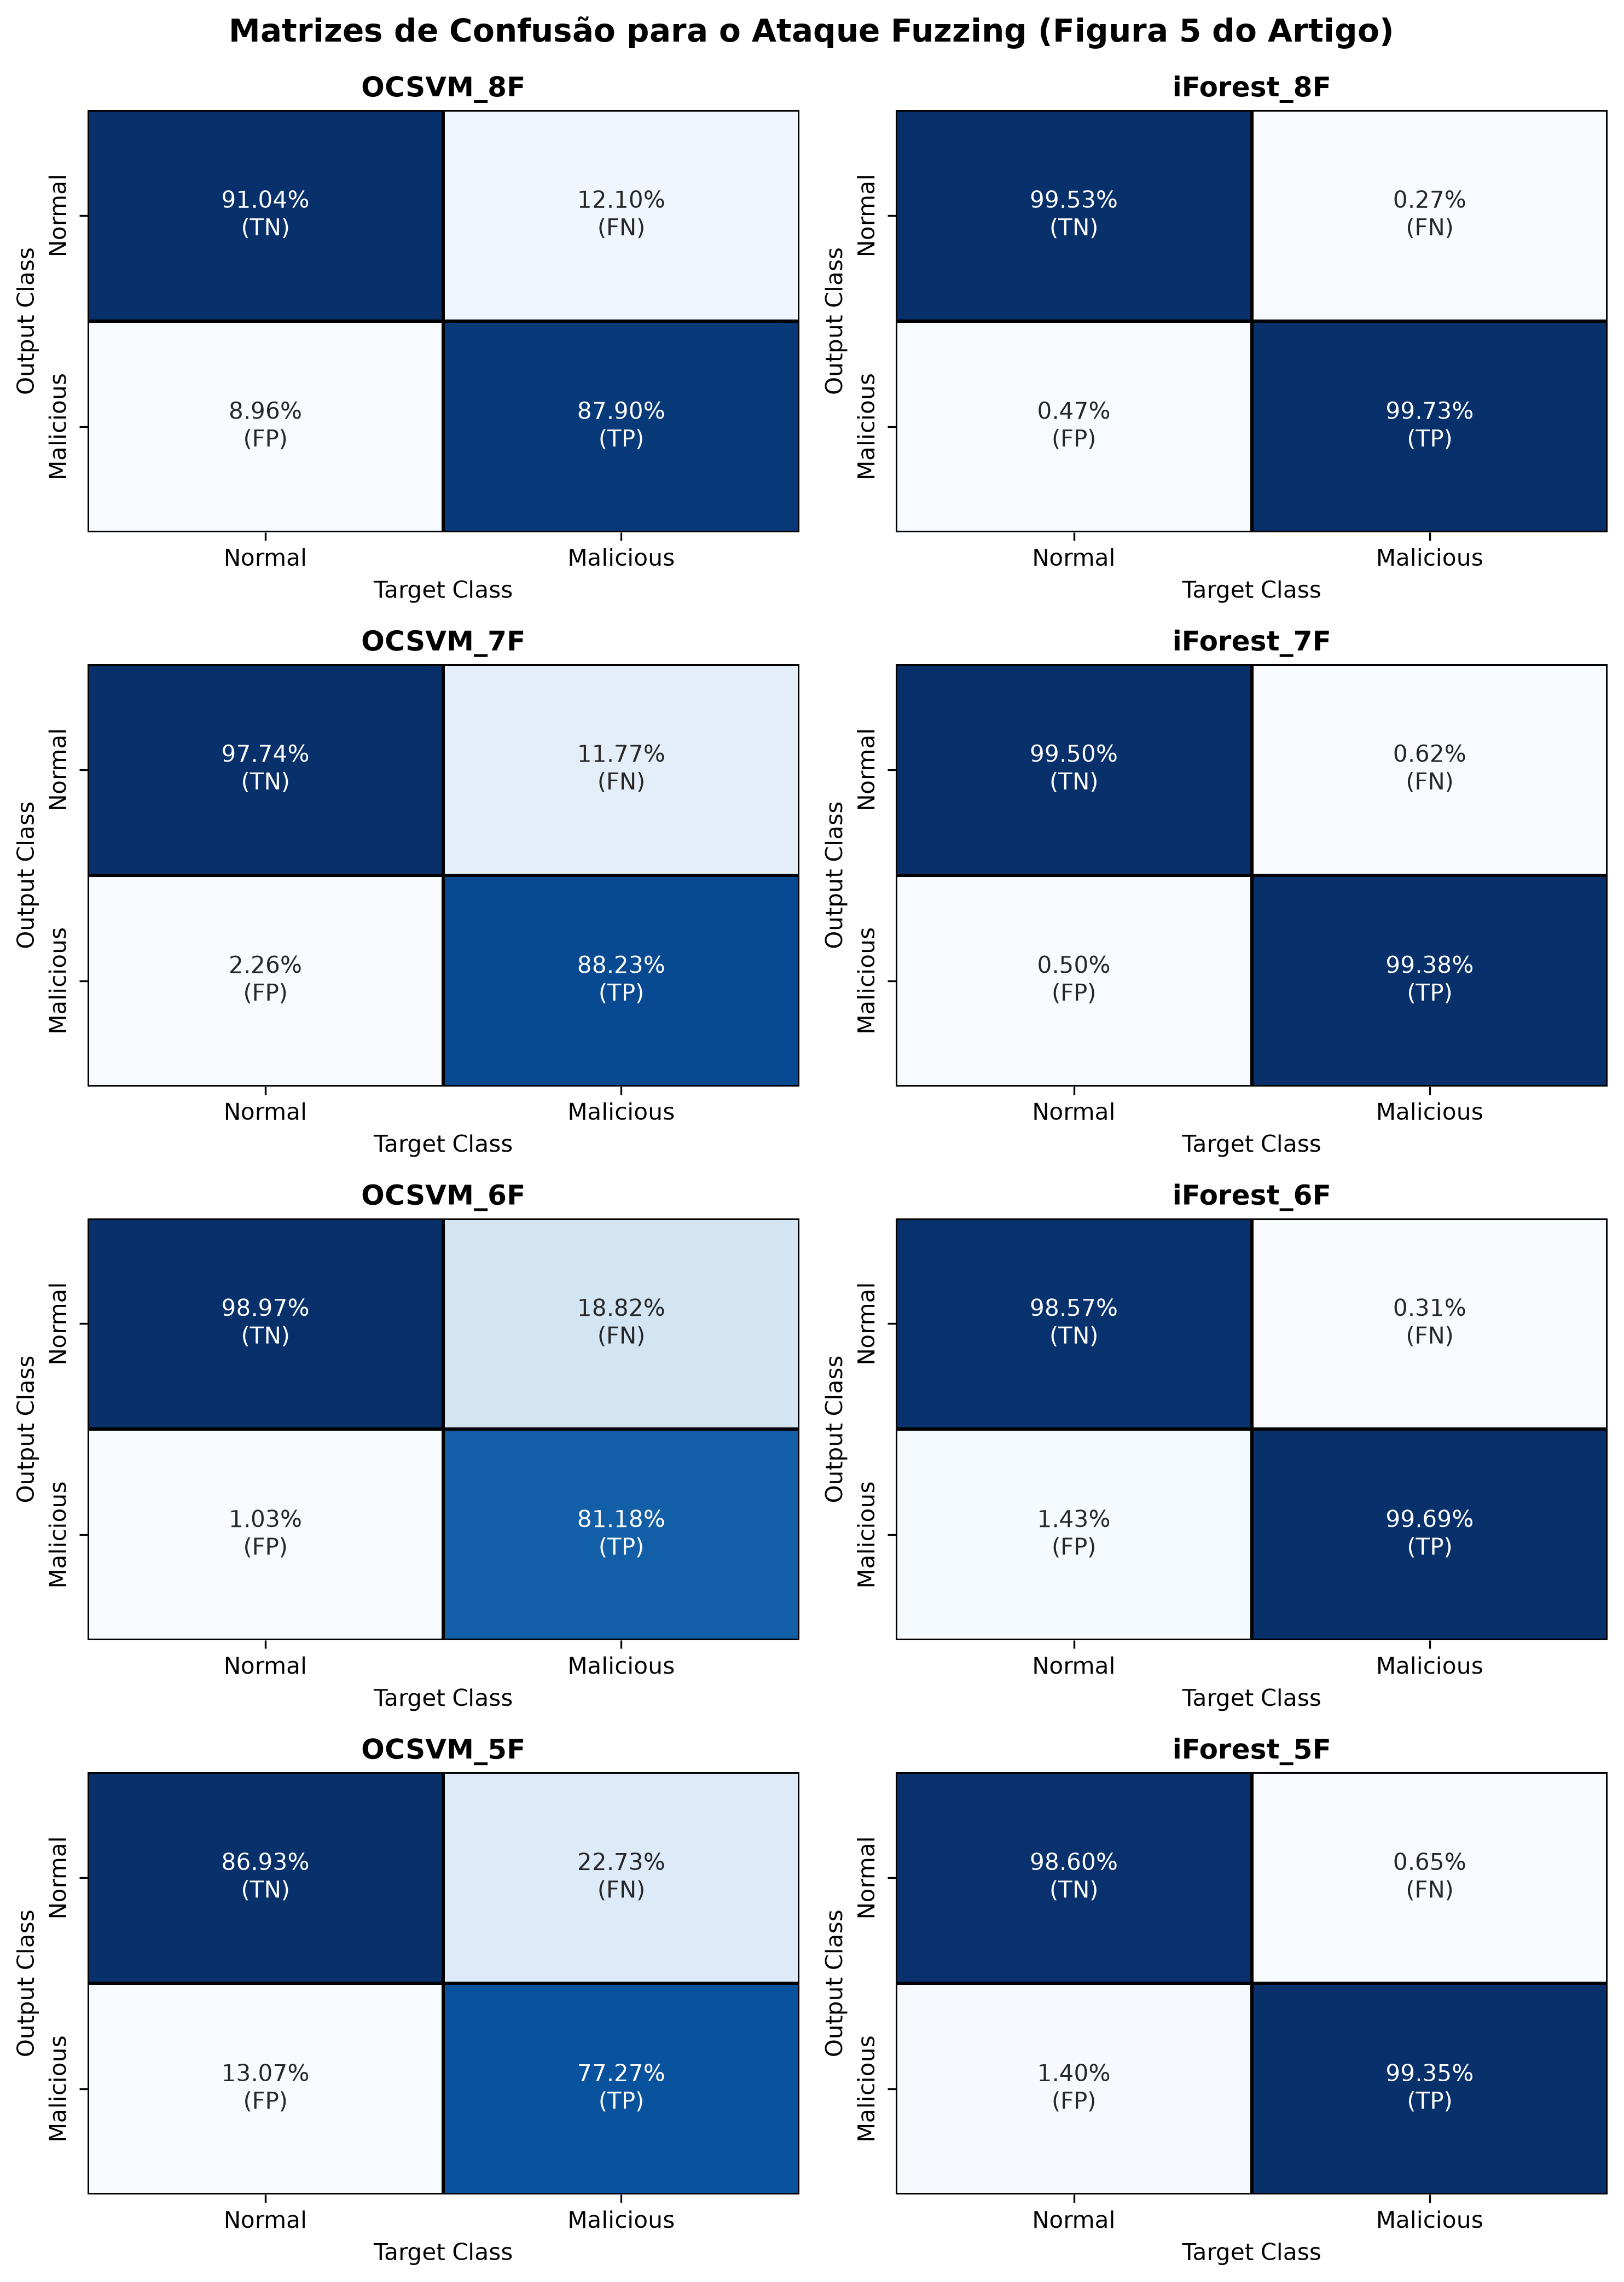
\includegraphics[width=0.98\columnwidth]{figure5_confusion_matrices.png}
\caption{Matrizes de confusão normalizadas por classe para os modelos OCSVM e iForest de 5 a 8 bytes no dataset Fuzzing (Reprodução da Figura 5 do Artigo).}
\label{fig:fig5_cm}
\end{figure}

\subsection{Comparação Estatística de Modelos (ANOVA, Tukey HSD e TOST)}
Na avaliação estatística sobre os 10 \textit{folds} de validação cruzada (ressalvada a sobreposição de $9/10$ do treino entre \textit{folds}):
\begin{itemize}
    \item O teste de D'Agostino-Pearson apresentou $p > 0{,}05$ para 14/16 modelos no \textit{Fuzzing}, 10/16 no \textit{Drive Gear} e 7/16 no \textit{RPM Gauge};
    \item O teste One-Way ANOVA indicou forte divergência global nos três datasets: $F = 226{,}26$ ($p = 5{,}24 \times 10^{-92}$) no \textit{Fuzzing}, $F = 1256{,}06$ ($p = 1{,}90 \times 10^{-144}$) no \textit{Drive Gear} e $F = 825{,}74$ ($p = 1{,}82 \times 10^{-131}$) no \textit{RPM Gauge};
    \item Pelo critério de Tukey HSD ($p > 0{,}05$ contra $\text{iForest\_8F}$) combinado ao teste pareado TOST ($\Delta = \pm 1{,}00\%$ p.p.): (i) no \textit{Fuzzing}, embora Tukey não detecte diferença significativa para $N \ge 3$ ($p \ge 0{,}5964$), o teste TOST revela que $\text{iForest\_3F}$ ($-2{,}63\%$, $p_{\text{TOST}}=0{,}9998$) e $\text{iForest\_4F}$ ($-2{,}17\%$, $p_{\text{TOST}}=0{,}9999$) ficam fora da margem de $\pm 1\%$, tornando \textbf{$\text{iForest\_5F}$} ($-0{,}76\%$, $\text{IC}_{90\%} [-0{,}93\%, -0{,}60\%]$, $p=1{,}0000$, $p_{\text{TOST}}=0{,}0134$) o menor modelo formalmente equivalente a $\text{iForest\_8F}$; (ii) no \textit{RPM Gauge}, $\text{iForest\_5F}$ ($-0{,}53\%$, $p=1{,}0000$, $\text{IC}_{90\%} [-0{,}93\%, -0{,}14\%]$, $p_{\text{TOST}}=0{,}0290$) também confirma equivalência dentro de $\pm 1\%$; e (iii) no \textit{Drive Gear}, os modelos de 1 a 3 bytes ficam abaixo de 85\% e são descartados, $\text{iForest\_4F}/\text{5F}$ diferem em validação ($p \le 0{,}0003$), e a equivalência TOST ocorre em $N \ge 6$ ($\text{iForest\_6F}$: $+0{,}19\%$, $p_{\text{TOST}}=7{,}50 \times 10^{-7}$), enquanto $\text{iForest\_5F}$ é adotado pela restrição física de~\eqref{eq:limit86} e salta para $98{,}32\%$ com $100\%$ de \textit{Recall} no conjunto de teste blindado.
\end{itemize}
Portanto, ratifica-se a escolha de $\text{iForest\_5F}$ como compromisso operacional unificado para compor o IPS em tempo real, conciliando equivalência prática dentro de $\pm 1\%$ em \textit{Fuzzing}/\textit{RPM Gauge} (e $100\%$ de \textit{Recall} em \textit{Drive Gear}) com a restrição física de $N \le 5$ bytes.

\subsection{Confronto com o Estado da Arte nos Três Datasets (Tabelas 9, 10 e 11)}
A Tabela~\ref{tab:sota_comparison} consolida as métricas reportadas nas Tabelas 9, 10 e 11 do artigo de referência (não re-executadas localmente neste projeto), confrontando-as com nossa replicação do $\text{iForest\_5F}$ e com o melhor modelo geral obtido em cada dataset frente aos quatro IDSs do estado da arte (GIDS \cite{seo2018gids}, DCNN \cite{song2020invehicle}, LSTM-IDS \cite{song2020invehicle} e MTH-IDS \cite{yang2021mth}).

\begin{table}[htbp]
\caption{Comparativo nos Três Datasets Frente a Métricas Reportadas na Literatura (Tabelas 9, 10 e 11 de \cite{araujo2021efficient})}
\label{tab:sota_comparison}
\centering
\scriptsize
\setlength{\tabcolsep}{3pt}
\begin{tabular}{llcccc}
\toprule
\textbf{Dataset} & \textbf{Mecanismo} & \textbf{Acc (\%)} & \textbf{Prec (\%)} & \textbf{Rec (\%)} & \textbf{F1 (\%)} \\
\midrule
\multirow{7}{*}{\textbf{Fuzzing}} 
 & GIDS \cite{seo2018gids} & 98,00 & 97,30 & 99,50 & 98,39 \\
 & DCNN \cite{song2020invehicle} & 99,82 & 99,95 & 99,65 & 99,80 \\
 & LSTM-based IDS \cite{song2020invehicle} & 99,35 & 99,36 & 99,16 & 99,26 \\
 & MTH-IDS \cite{yang2021mth} & 99,99 & 99,99 & 99,99 & 99,99 \\
 & \textbf{IPS Proposto (Artigo)} & \textbf{99,29} & \textbf{95,07} & \textbf{99,93} & \textbf{97,44} \\
 & \textbf{Replicação (iForest\_5F)} & \textbf{98,70} & \textbf{91,66} & \textbf{99,35} & \textbf{95,35} \\
 & \textbf{Replicação (iForest\_8F)} & \textbf{99,55} & \textbf{97,03} & \textbf{99,73} & \textbf{98,36} \\
\midrule
\multirow{7}{*}{\textbf{Drive Gear}} 
 & GIDS \cite{seo2018gids} & 96,20 & 98,10 & 96,50 & 97,29 \\
 & DCNN \cite{song2020invehicle} & 99,95 & 99,99 & 99,89 & 99,94 \\
 & LSTM-based IDS \cite{song2020invehicle} & 99,76 & 99,75 & 99,68 & 99,72 \\
 & MTH-IDS \cite{yang2021mth} & 99,99 & 99,99 & 99,99 & 99,99 \\
 & \textbf{IPS Proposto (Artigo)} & \textbf{99,24} & \textbf{94,79} & \textbf{100,00} & \textbf{97,33} \\
 & \textbf{Replicação (iForest\_5F)} & \textbf{98,32} & \textbf{89,20} & \textbf{100,00} & \textbf{94,29} \\
 & \textbf{Replicação (iForest\_6F)} & \textbf{99,57} & \textbf{96,96} & \textbf{100,00} & \textbf{98,46} \\
\midrule
\multirow{7}{*}{\textbf{RPM Gauge}} 
 & GIDS \cite{seo2018gids} & 98,00 & 98,30 & 99,00 & 98,65 \\
 & DCNN \cite{song2020invehicle} & 99,97 & 99,99 & 99,94 & 99,96 \\
 & LSTM-based IDS \cite{song2020invehicle} & 99,87 & 100,00 & 99,71 & 99,85 \\
 & MTH-IDS \cite{yang2021mth} & 99,99 & 99,99 & 99,99 & 99,99 \\
 & \textbf{IPS Proposto (Artigo)} & \textbf{99,85} & \textbf{98,97} & \textbf{100,00} & \textbf{99,48} \\
 & \textbf{Replicação (iForest\_5F)} & \textbf{99,14} & \textbf{94,47} & \textbf{100,00} & \textbf{97,15} \\
 & \textbf{Replicação (iForest\_8F)} & \textbf{99,58} & \textbf{97,22} & \textbf{100,00} & \textbf{98,59} \\
\bottomrule
\end{tabular}
\end{table}

Os resultados da Tabela~\ref{tab:sota_comparison} evidenciam que a nossa replicação do $\text{iForest\_5F}$ supera a acurácia do GIDS nos três conjuntos de dados ($98{,}70\%$ vs. $98{,}00\%$ no \textit{Fuzzing}; $98{,}32\%$ vs. $96{,}20\%$ no \textit{Drive Gear}; e $99{,}14\%$ vs. $98{,}00\%$ no \textit{RPM Gauge}), atingindo $100{,}00\%$ de \textit{Recall} nos dois ataques de \textit{Spoofing} e $99{,}35\%$ no \textit{Fuzzing}. Embora abordagens supervisionadas (DCNN e LSTM-IDS) e híbridas (MTH-IDS) alcancem F1-Scores ligeiramente superiores ($99{,}80\%\text{--}99{,}99\%$), elas não conseguem descartar quadros maliciosos antes do término da transmissão, ao passo que o IPS baseado em $\text{iForest\_5F}$ previne ativamente que os ataques alcancem as ECUs.

\subsection{Resultados no Segundo Conjunto de Dados: Speedometer Spoofing}
Utilizando exatamente a grade completa (\texttt{full}) expandida com as combinações campeãs do grid refinado, executou-se o treinamento e a avaliação dos 16 modelos ($\text{iForest\_1F}\dots\text{8F}$ e $\text{OCSVM\_1F}\dots\text{8F}$) sobre o dataset \textit{Speedometer}. A Tabela~\ref{tab:speedometer_results} e a Fig.~\ref{fig:speedometer_analysis} consolidam os resultados obtidos na validação cruzada e no conjunto de teste blindado ($118.046$ quadros).

\begin{table}[htbp]
\caption{Desempenho dos 16 Modelos no Dataset Speedometer Spoofing (Teste Blindado: 118.046 Quadros)}
\label{tab:speedometer_results}
\centering
\scriptsize
\setlength{\tabcolsep}{2.5pt}
\begin{tabular}{lcccccc}
\toprule
\textbf{Modelo} & \textbf{Val (\%)} & \textbf{Acc (\%)} & \textbf{Prec (\%)} & \textbf{Rec (\%)} & \textbf{F1 (\%)} & \textbf{AUC (\%)} \\
\midrule
\textbf{iForest\_3F} & \textbf{99,48} & \textbf{99,12} & \textbf{75,97} & \textbf{100,00} & \textbf{86,34} & \textbf{99,64} \\
iForest\_4F & 97,30 & 95,48 & 38,00 & 100,00 & 55,07 & 98,41 \\
iForest\_5F & 97,34 & 95,45 & 37,87 & 100,00 & 54,93 & 96,89 \\
iForest\_6F & 97,02 & 95,15 & 36,36 & 100,00 & 53,32 & 96,11 \\
iForest\_7F & 95,54 & 90,71 & 22,98 & 100,00 & 37,37 & 92,86 \\
iForest\_8F & 95,38 & 90,88 & 23,31 & 100,00 & 37,81 & 92,92 \\
iForest\_2F & 87,40 & 76,91* & 10,72 & 100,00 & 19,36 & 80,67 \\
iForest\_1F & 93,38 & 87,57 & 18,23 & 100,00 & 30,84 & 90,45 \\
\midrule
\textbf{OCSVM\_4F} & \textbf{96,50} & \textbf{97,23} & \textbf{50,05} & \textbf{100,00} & \textbf{66,71} & \textbf{100,00} \\
OCSVM\_8F & 95,48 & 82,59* & 13,74 & 100,00 & 24,16 & 100,00 \\
OCSVM\_6F & 98,40 & 81,69* & 13,15 & 100,00 & 23,24 & 100,00 \\
OCSVM\_3F & 97,16 & 82,44* & 13,63 & 100,00 & 24,00 & 100,00 \\
OCSVM\_7F & 96,74 & 80,96* & 12,71 & 100,00 & 22,55 & 100,00 \\
OCSVM\_5F & 96,86 & 77,12* & 10,80 & 100,00 & 19,50 & 99,51 \\
OCSVM\_2F & 49,82* & 96,88 & 0,00 & 0,00 & 0,00 & 3,22 \\
OCSVM\_1F & 49,92* & 96,88 & 0,00 & 0,00 & 0,00 & 28,09 \\
\bottomrule
\multicolumn{7}{l}{\tiny *Acurácia $<85\%$ na validação ou no teste (ou Recall nulo).}
\end{tabular}
\end{table}

\begin{figure}[htbp]
\centering
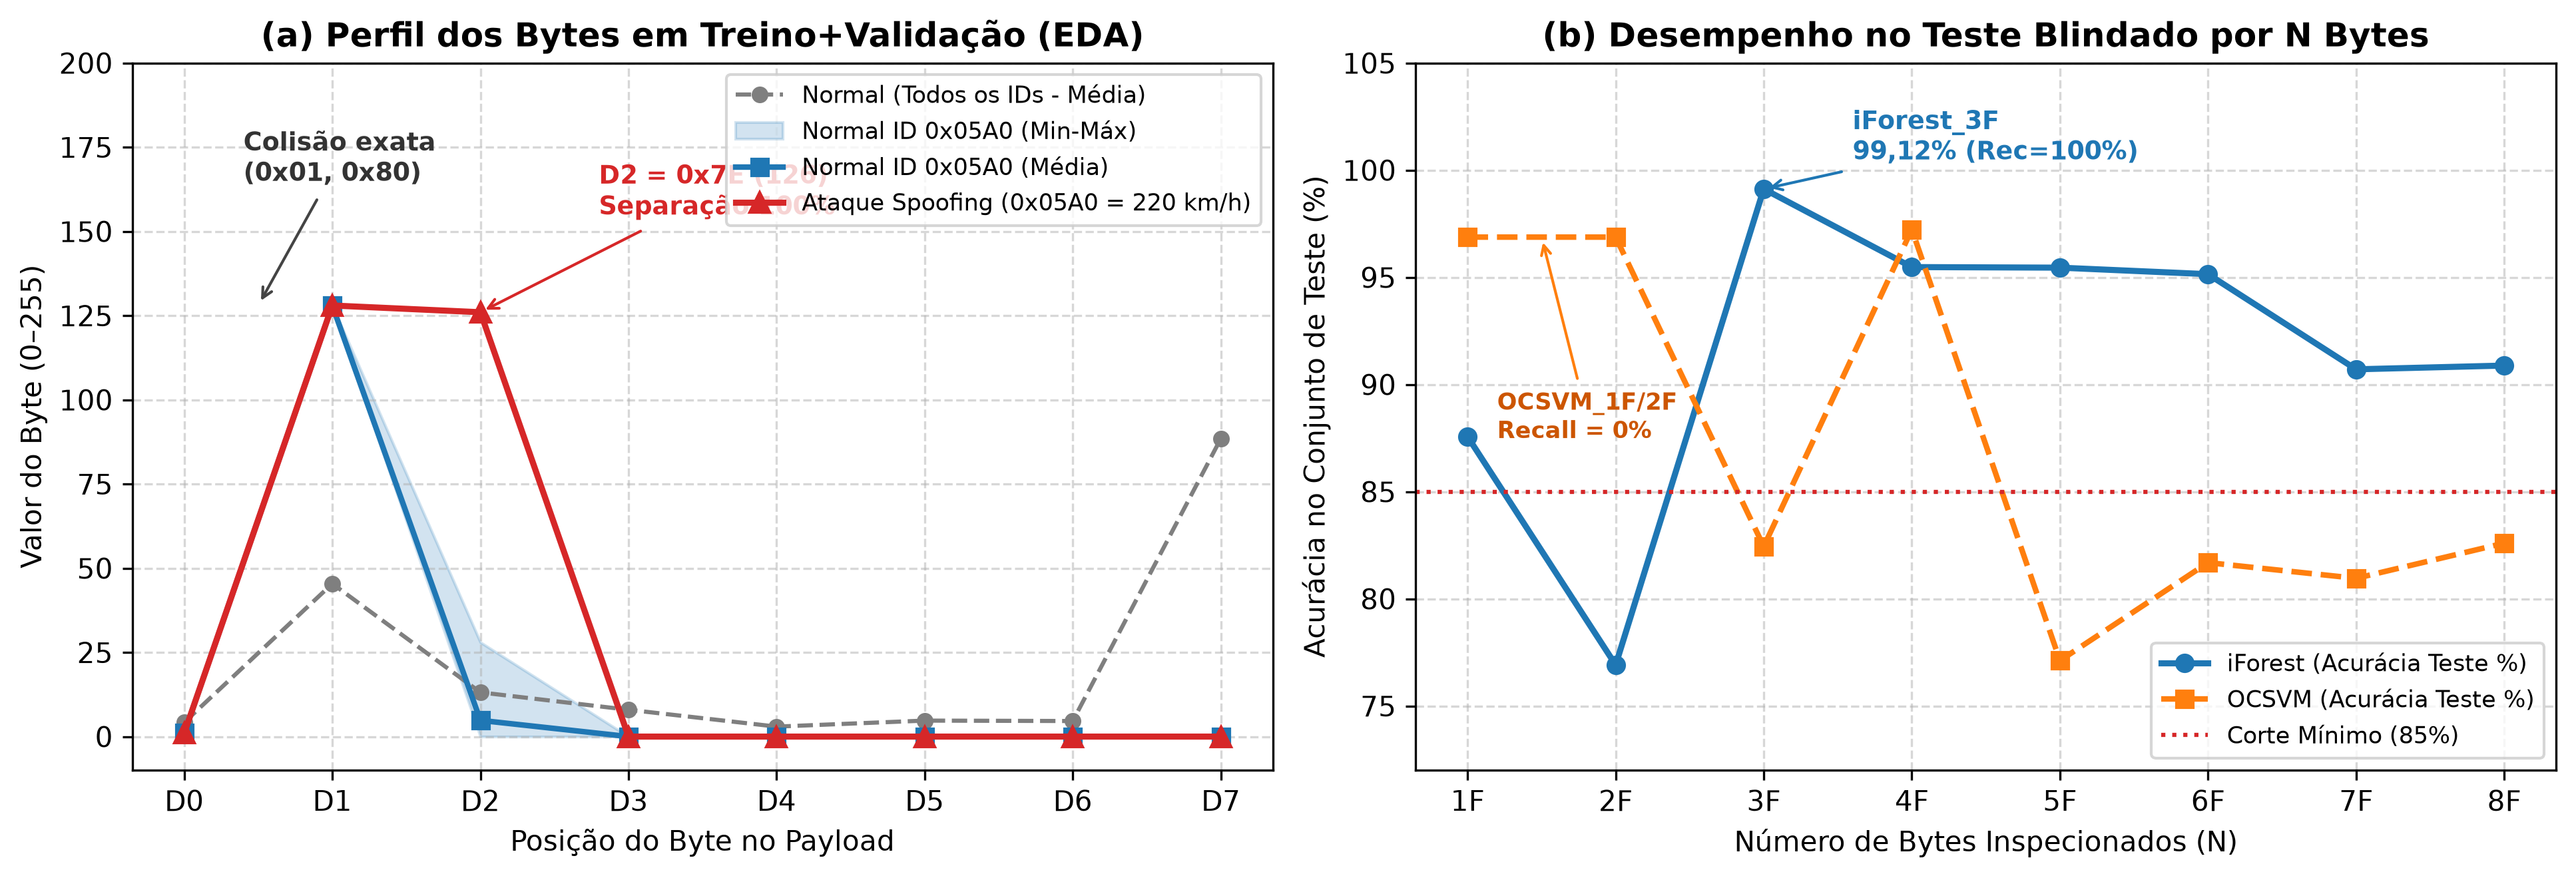
\includegraphics[width=0.98\columnwidth]{fig_speedometer_analysis.png}
\caption{Análise do segundo conjunto de dados (\textit{Speedometer Spoofing}): (a) perfil dos bytes $D_0 \dots D_7$ em Treino+Validação mostrando a colisão exata em $D_0, D_1$ e a separação em $D_2 = \texttt{0x7E}$; (b) acurácia no teste blindado em função de $N$.}
\label{fig:speedometer_analysis}
\end{figure}

Na análise estatística sobre os 10 \textit{folds}, $11/16$ modelos (incluindo todos os 8 modelos \textit{iForest}) satisfizeram $p > 0{,}05$ em D'Agostino-Pearson e o One-Way ANOVA indicou divergência significativa ($F = 275{,}66, p = 6{,}22 \times 10^{-98}$). No teste de Tukey HSD, $\text{iForest\_3F}$ ($N \ge 3$ bytes) foi o menor candidato sem diferença bilateral detectada frente a $\text{iForest\_8F}$ ($p = 0{,}1774$), ao passo que o teste pareado TOST ($\Delta = \pm 1{,}00\%$ p.p.) revelou que $\text{iForest\_3F}$ na realidade \emph{supera} $\text{iForest\_8F}$ em $+4{,}10\%$ na média dos \textit{folds} ($\text{IC}_{90\%} [+3{,}46\%, +4{,}74\%]$, $p_{\text{TOST}}=1{,}00$), confirmando ganho líquido sobre o modelo de 8 bytes. Os resultados revelam três conclusões importantes:
\begin{enumerate}
    \item \textbf{Confirmação empírica da fronteira em $N=3$ bytes:} Para $N \le 2$ bytes, os quadros de ataque são idênticos ao prefixo normal \texttt{01 80} de \texttt{0x05A0}, levando $\text{OCSVM\_1F}/\text{2F}$ a $0{,}00\%$ de \textit{Recall} e $\text{iForest\_2F}$ a $76{,}91\%$ de acurácia. Ao incluir o 3º byte ($D_2 = \texttt{0x7E}$), o modelo $\text{iForest\_3F}$ (\texttt{contamination=0.01, max\_samples=512, n\_estimators=200}) atinge \textbf{99,12\% de acurácia}, \textbf{100,00\% de Recall}, \textbf{99,64\% de AUC-ROC} e apenas $0{,}90\%$ de falsos positivos;
    \item \textbf{Efeito de diluição por bytes redundantes ($N > 3$):} Ao contrário do \textit{Car-Hacking}, onde múltiplos bytes iniciais diferiam do normal, no \textit{Speedometer} os bytes $D_3 \dots D_7$ são todos \texttt{0x00} (idênticos a $>93\%$ do barramento normal). Adicionar essas dimensões reduz a probabilidade de cada árvore sortear $D_2$ de $1/3$ em $\text{iForest\_3F}$ para $1/5$ em $\text{iForest\_5F}$ ($95{,}45\%$) e $1/8$ em $\text{iForest\_8F}$ ($90{,}88\%$), ratificando que inspecionar menos bytes também melhora a relação sinal-ruído;
    \item \textbf{Sensibilidade da validação balanceada e escopo do valor fixo:} Como o conjunto de teste real possui $97{,}23\%$ de quadros normais, configurações selecionadas com $\texttt{contamination} \in \{0{,}05, 0{,}1\}$ ou $\nu \ge 0{,}02$ na validação balanceada elevaram os falsos positivos no teste (reduzindo a precisão para $13\%\text{--}38\%$). Ademais, embora $\text{iForest\_3F}$ detecte integralmente o ataque a $220\,\text{km/h}$ ($\texttt{0x7E}$), um ataque de \textit{Spoofing} que injetasse uma velocidade dentro da faixa urbana normal ($D_2 \in [0, 28]$) evadiria modelos baseados unicamente em bytes sem $\Delta t$ e \textit{CAN ID}.
\end{enumerate}

\section{Proposta de Melhoria e Prova de Conceito: IPS em Dois Estágios com Dual-Cache}

Embora a arquitetura $\text{iForest\_5F}$ atinja alta eficácia dentro do limite de tempo real de~\eqref{eq:limit86}, taxas residuais de falsos positivos entre $0{,}5\%$ e $1{,}4\%$ comprometem a disponibilidade do barramento CAN sob ataque ou operação intensa. Para mitigar esse problema sem abdicar do bloqueio imediato, propomos e implementamos uma extensão arquitetural em dois estágios com memória compartilhada em três \textit{threads} e sistema \textit{Dual-Cache}.

\subsection{Motivação Protocolar: Modelo de Confinamento de Erros e Risco de Bus-Off}
De acordo com o mecanismo de confinamento de erros da especificação CAN 2.0A~\cite{bosch1991can,kvaser_error}, cada módulo mantém um contador de erros de transmissão (\textit{Transmit Error Counter} -- \textit{TEC}). Quando o IPS descarta um quadro legítimo ao injetar um \textit{Active Error Frame} no 5º byte, a ECU emissora incrementa $\text{TEC} \mathrel{+}= 8$ e realiza retransmissão automática (parametrizada no modelo em janelas de $260~\mu\text{s}$ a $500\text{ kbps}$). Apenas transmissões concluídas com sucesso decrementam $\text{TEC} \mathrel{-}= 1$.

Como os logs públicos não fornecem matriz DBC de mapeamento ECU--identificador, modelamos em \texttt{poc\_ips/poc\_simulator.py} uma máquina de estados TEC independente por \texttt{CAN\_ID} atuando como \textit{proxy} de ECU, por meio de um modelo simplificado de eventos orientado a traços cronológicos (sem reescalonamento global de arbitragem no barramento). Como o modelo $\text{iForest\_5F}$ é determinístico e \textit{stateless}, toda retransmissão automática reproduz os mesmos 5 primeiros bytes e sofre novo descarte imediato: $12$ aborts conduzem a \textit{Error Warning} ($\text{TEC} \ge 96$), $16$ a \textit{Error Passive} ($\text{TEC} > 127$) e $32$ retransmissões abortadas consecutivamente ($32 \times 8 = 256 > 255$) levam ao estado \textit{Bus-Off}, gerando indisponibilidade da unidade até sua recuperação (assumida em parâmetro nominal de $50\text{ ms}$, contrastada na análise de sensibilidade ao mínimo físico CAN 2.0A de $128 \times 11$ bits recessivos $\approx 2{,}8\text{ ms}$ a $500\text{ kbps}$).

\subsection{Arquitetura em Dois Estágios, Dual-Cache e Três Threads}
Para interromper essa cascata de falsos positivos sem extrapolar a janela crítica de~\eqref{eq:limit86} ($86~\mu\text{s}$), projetamos a arquitetura concorrente em três \textit{threads} descrita a seguir:
\begin{enumerate}
    \item \textbf{Estágio 1 ($\text{iForest\_5F}$, \textit{Worker\_Stage1}):} Mantém o modelo de 5 bytes pré-carregado em memória compartilhada para eliminar a sobrecarga de inicialização de processos e responder de forma síncrona à chegada de $[D_0 \dots D_4]$. Quadros anômalos inéditos (como pacotes aleatórios de \textit{Fuzzing}) continuam bloqueados imediatamente no barramento;
    \item \textbf{Estágio 2 Assíncrono ($\text{CAN\_ID} + 8\text{ bytes}$, \textit{Worker\_Stage2}):} Como o algoritmo OCSVM apresentou desempenho sistematicamente inferior nos experimentos base, restringimos o Estágio 2 exclusivamente ao \textit{Isolation Forest}, incorporando o identificador normalizado ($\text{CAN\_ID}/2047$ no espaço padrão de $11\text{ bits}$) e o campo de dados completo ($D_0 \dots D_7$). Avaliamos três variantes: (i) $\text{iForest\_9F\_Global}$ (floresta global de $9$ atributos); (ii) $\text{iForest\_Hybrid\_Fallback}$ (florestas locais de $8$ bytes por \textit{CAN ID} quando há $\ge 10$ amostras no treino, com \textit{fallback} para o modelo $9\text{F}$ global em IDs raros ou inéditos); e (iii) $\text{iForest\_Hybrid\_StrictUnknown}$ (tratamento estritamente suspeito para IDs nunca vistos). A inferência em C de ambos os estágios foi verificada pela suíte executável \texttt{poc\_ips/test\_equivalence.py} contra o \texttt{scikit-learn}, obtendo diferença máxima de escore $\le 1{,}11 \times 10^{-16}$ e $0$ divergências de predição em amostras de teste reais e de fronteira;
    \item \textbf{Coordenador e Sistema \textit{Dual-Cache} (\textit{Coordinator}):} Recebe os 8 bytes do quadro, indexados em $\mathcal{O}(1)$ por uma chave inteira compacta de $75\text{ bits}$ dada por $(\text{CAN\_ID} \ll 64) \mid \text{payload}_{64}$, e gerencia duas caches em memória:
    \begin{itemize}
        \item \textit{Cache 1 (Suspeitos / Deduplicação):} Contabiliza ocorrências suspeitas sinalizadas pelo Estágio 1 ($\text{status} \in \{\texttt{OBSERVING}, \texttt{PENDING}\}$). Ao atingir o limiar de disparo $k_{\text{trig}}$ ($k_{\text{trig}}=1$ no modelo proposto), envia o quadro assincronamente ao \textit{Worker\_Stage2} (orçamento simulado de conclusão pós-8º byte de $200~\mu\text{s}$), evitando reenvios redundantes em rajadas enquanto a análise está pendente;
        \item \textit{Cache 2 (Cache de Vereditos com Expiração Temporal):} Armazena o veredicto definitivo (\texttt{ALLOW} ou \texttt{BLOCK}) do Estágio 2 com janela de validade $\text{TTL} = 100\text{ ms}$, imposta via invalidação preguiçosa a cada consulta (\textit{lazy lookup}) e varredura periódica a cada $50.000$ quadros. Em qualquer retransmissão subsequente da ECU ou novo ciclo dentro de $100\text{ ms}$, o Coordenador responde em $\mathcal{O}(1)$ sem reacionar o Estágio 1 — interrompendo cascatas de \textit{Bus-Off} — enquanto o \textit{TTL} limita o consumo de RAM e a janela de permanência do veredicto (ressaltando-se que repetições maliciosas idênticas dentro dos $100\text{ ms}$ acertam a Cache 2 sem defesa \textit{anti-replay}).
    \end{itemize}
\end{enumerate}

\subsection{Desempenho do Estágio 2 (CAN\_ID + 8 Bytes) em Validação Cruzada}
Cada variante do Estágio 2 foi submetida à mesma validação cruzada de 10 \textit{folds} isenta de vazamento de dados e à mesma grade completa de hiperparâmetros da replicação base (\textit{iForest}-only). A Tabela~\ref{tab:stage2_cv_test} e a Fig.~\ref{fig:stage2_cascade} resumem os resultados da avaliação em cascata ($\text{Estágio 1} \rightarrow \text{Estágio 2}$) sobre os conjuntos de teste cegos ($12.027.273$ quadros no total).

\begin{table}[htbp]
\caption{Desempenho do Estágio 2 e Resgate de Falsos Positivos em Cascata nos Conjuntos de Teste}
\label{tab:stage2_cv_test}
\centering
\scriptsize
\setlength{\tabcolsep}{1.5pt}
\begin{tabular}{llcccccc}
\toprule
\textbf{Dataset} & \textbf{Modelo} & \textbf{Acc(\%)} & \textbf{Prec(\%)} & \textbf{Rec(\%)} & \textbf{F1(\%)} & \textbf{FP} & \textbf{Resg.} \\
\midrule
\multirow{3}{*}{\textbf{Fuzzing}} 
 & 5F (Base) & 98,70 & 91,66 & \textbf{99,35} & 95,35 & 42.200 & --- \\
 & \textbf{9F\_Global*} & \textbf{99,71} & \textbf{98,90} & 98,95 & \textbf{98,92} & \textbf{5.143} & \textbf{87,81\%} \\
 & Hybrid\_FB & 99,55 & 97,79 & 98,87 & 98,32 & 10.442 & 75,26\% \\
\midrule
\multirow{3}{*}{\textbf{Drive G.}} 
 & 5F (Base) & 98,32 & 89,20 & 100,00 & 94,29 & 69.314 & --- \\
 & 9F\_Global & 99,49 & 96,46 & 100,00 & 98,20 & 20.993 & 69,71\% \\
 & \textbf{Hybrid\_FB*} & \textbf{99,87} & \textbf{99,08} & \textbf{100,00} & \textbf{99,54} & \textbf{5.287} & \textbf{92,37\%} \\
\midrule
\multirow{3}{*}{\textbf{RPM G.}} 
 & 5F (Base) & 99,14 & 94,47 & 100,00 & 97,15 & 36.892 & --- \\
 & 9F\_Global & 99,79 & 98,56 & 100,00 & 99,28 & 9.181 & 75,11\% \\
 & \textbf{Hybrid\_FB*} & \textbf{99,89} & \textbf{99,27} & \textbf{100,00} & \textbf{99,64} & \textbf{4.606} & \textbf{87,51\%} \\
\midrule
\multirow{3}{*}{\textbf{Speedom.}} 
 & 5F (Base) & 95,45 & 37,87 & 100,00 & 54,93 & 5.369 & --- \\
 & 9F\_Global & 95,45 & 37,87 & 100,00 & 54,93 & 5.369 & 0,00\% \\
 & \textbf{Hybrid\_FB*} & \textbf{97,88} & \textbf{56,68} & \textbf{100,00} & \textbf{72,35} & \textbf{2.501} & \textbf{53,42\%} \\
\bottomrule
\multicolumn{8}{l}{\tiny *Vencedor na CV 10-\textit{folds} (\texttt{Hybrid\_FB} = \texttt{iForest\_Hybrid\_Fallback}).}
\end{tabular}
\end{table}

\begin{figure}[htbp]
\centering
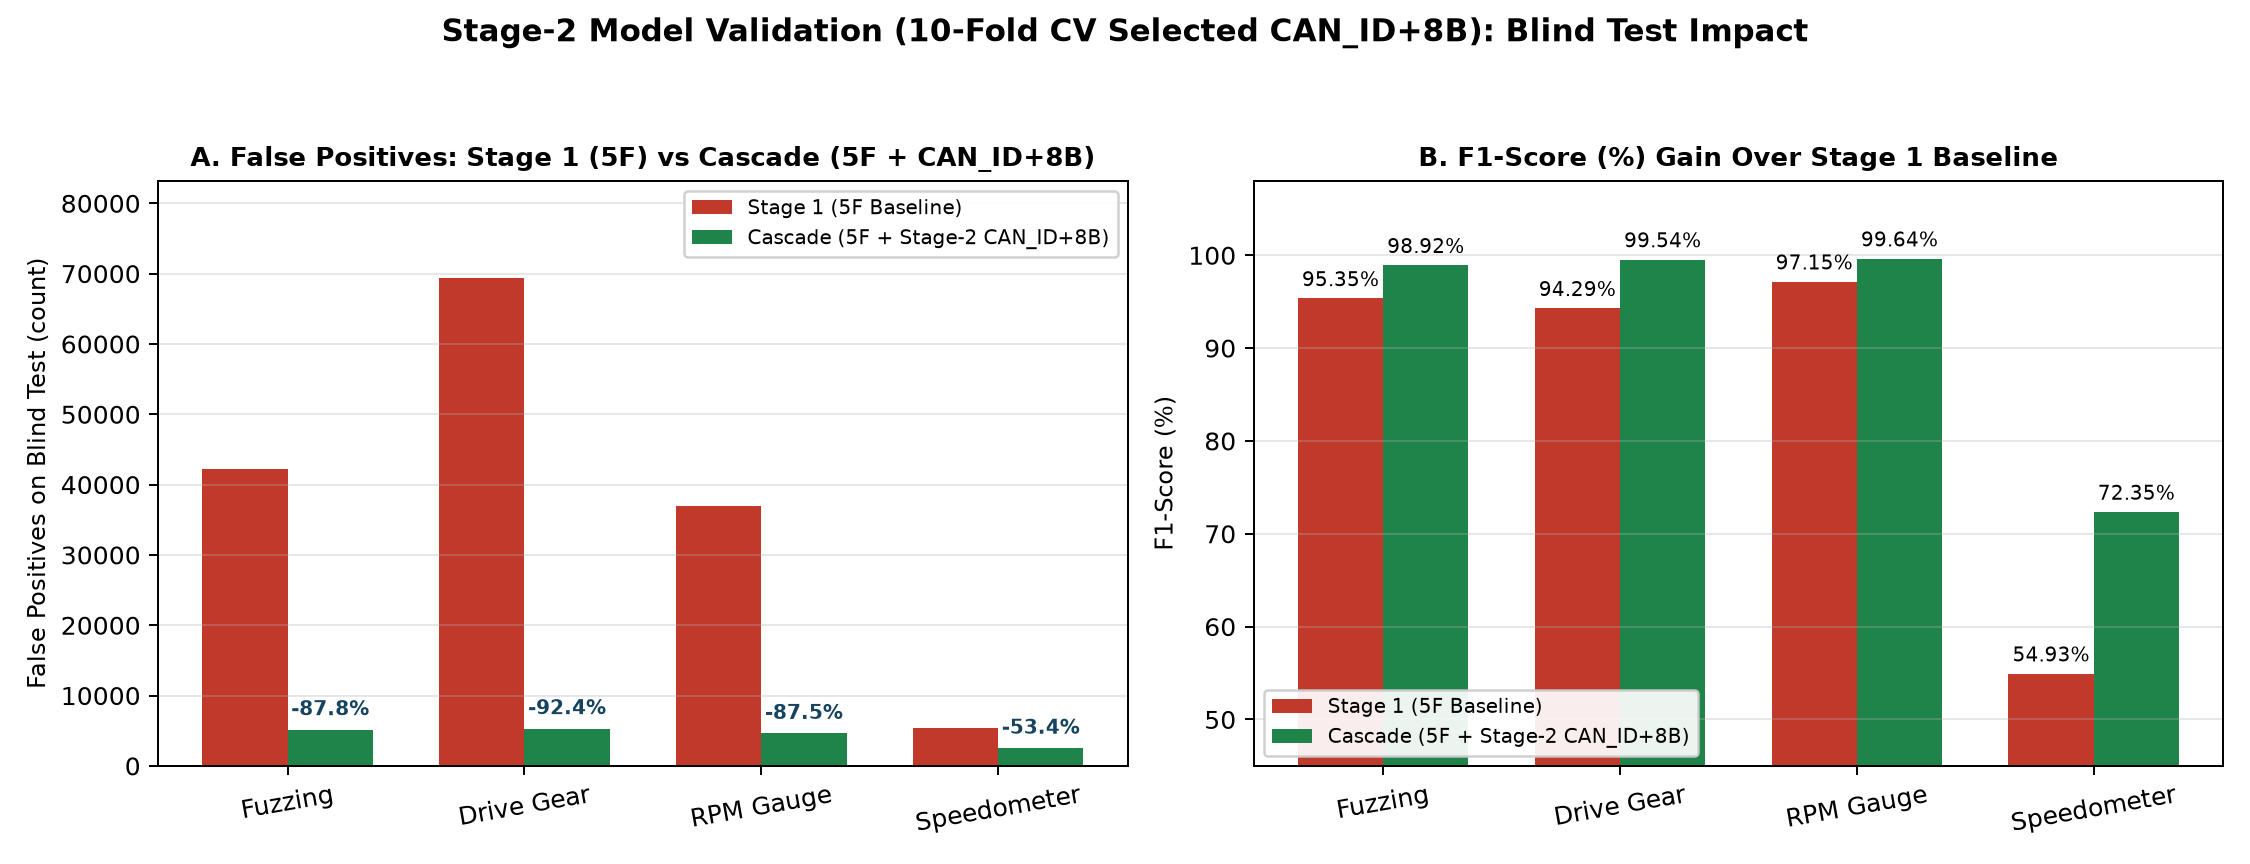
\includegraphics[width=0.98\columnwidth]{fig_stage2_cascade.png}
\caption{Comparativo do Estágio 2 em cascata: (a) porcentagem de falsos positivos de 5 bytes resgatados sem degradação nos ataques e (b) ganho de F1-Score sobre o \textit{baseline} $\text{iForest\_5F}$.}
\label{fig:stage2_cascade}
\end{figure}

Os resultados revelam uma distinção estrutural clara entre ataques de \textit{Spoofing} e \textit{Fuzzing}:
\begin{itemize}
    \item Nos ataques de \textit{Spoofing} (\textit{Drive Gear}, \textit{RPM Gauge} e \textit{Speedometer}), a variante $\text{iForest\_Hybrid\_Fallback}$ venceu a validação cruzada ($99{,}85\%$, $99{,}87\%$ e $97{,}76\%$ de acurácia média de CV) e resgatou $\mathbf{92{,}37\%}$, $\mathbf{87{,}51\%}$ e $\mathbf{53{,}42\%}$ dos falsos positivos do modelo de 5 bytes, preservando \textbf{100,00\% de Recall} ($0$ falsos negativos). Em particular, no \textit{Speedometer}, onde um modelo $9\text{F}$ global único não conseguiu isolar distribuições condicionadas por identificador ($0{,}00\%$ de resgate em cascata), o particionamento por \textit{CAN ID} elevou o F1-Score de $54{,}93\%$ para $72{,}35\%$. A variante $\text{Hybrid\_StrictUnknown}$ obteve métricas idênticas à $\text{Hybrid\_Fallback}$ nesses três cenários por não haver \textit{CAN IDs} inéditos no teste;
    \item No ataque de \textit{Fuzzing}, que injeta mensagens ao longo de todos os $2.048$ identificadores de $11\text{ bits}$, o $\text{iForest\_9F\_Global}$ destacou-se ($99{,}55\%$ em CV), resgatando $\mathbf{87{,}81\%}$ dos falsos positivos (reduzindo de $42.200$ para $5.143$) e elevando a acurácia em cascata para $99{,}71\%$ (com pequena perda de $0{,}41\%$ nos verdadeiros positivos na avaliação puramente estática, reduzindo o Recall de $99{,}35\%$ para $98{,}95\%$).
\end{itemize}

\subsection{Resultados da Prova de Conceito (3 Threads), Ablações e Sensibilidade}
Acoplamos o motor PoC em três \textit{threads} (com extensões em C pré-carregadas) ao modelo simplificado orientado a traços de confinamento de erros CAN 2.0A sobre os quatro fluxos de teste completos, comparando quatro configurações: (i) \texttt{Baseline\_5F} (apenas Estágio 1); (ii) \texttt{Proposed\_DualCache\_100ms} ($k_{\text{trig}}=1$, $\text{TTL}=100\text{ ms}$); (iii) \texttt{Ablation\_Trigger2\_100ms} ($k_{\text{trig}}=2$, $\text{TTL}=100\text{ ms}$); e (iv) \texttt{Ablation\_DualCache\_NoTTL} ($k_{\text{trig}}=1$, sem expiração). Os resultados estão consolidados na Tabela~\ref{tab:poc_simulation} e ilustrados na Fig.~\ref{fig:poc_comparison}.

\begin{table*}[htbp]
\caption{Resultados no Modelo Simplificado de Confinamento de Erros CAN 2.0A por \texttt{CAN\_ID} (PoC em 3 Threads e Ablações)}
\label{tab:poc_simulation}
\centering
\scriptsize
\setlength{\tabcolsep}{3.5pt}
\begin{tabular}{llccccccr}
\toprule
\textbf{Dataset} & \textbf{Configuração} & \textbf{Aborts Legít.} & \textbf{Bus-Off} & \textbf{Red. Bus-Off} & \textbf{Norm. Perd.} & \textbf{Recall (\%)} & \textbf{Cham. E2} & \textbf{Hits C2} \\
\midrule
\multirow{4}{*}{\textbf{Speedometer}}
 & Baseline\_5F & 95.488 & 2.984 & --- & 22.736 & 100,00 & 0 & 0 \\
 & \textbf{Proposed\_DualCache\_100ms} & \textbf{34.644} & \textbf{1.064} & \textbf{-64,34\%} & \textbf{19.740} & \textbf{100,00} & 3.132 & 37.470 \\
 & Ablation\_Trigger2\_100ms & 36.162 & 1.111 & -62,77\% & 19.779 & 100,00 & 3.104 & 35.867 \\
 & Ablation\_DualCache\_NoTTL & 33.048 & 1.029 & -65,52\% & 19.713 & 100,00 & 540 & 38.497 \\
\midrule
\multirow{4}{*}{\textbf{Fuzzing}}
 & Baseline\_5F & 834.432 & 26.076 & --- & 94.979 & 99,35 & 0 & 0 \\
 & \textbf{Proposed\_DualCache\_100ms} & \textbf{129.313} & \textbf{3.338} & \textbf{-87,20\%} & \textbf{7.760} & \textbf{99,35} & 493.727 & 135.679 \\
 & Ablation\_Trigger2\_100ms & 152.913 & 3.602 & -86,19\% & 8.523 & 99,35 & 29.646 & 129.409 \\
 & Ablation\_DualCache\_NoTTL & 114.040 & 3.236 & -87,59\% & 7.522 & 99,35 & 475.720 & 138.584 \\
\midrule
\multirow{4}{*}{\textbf{Drive Gear}}
 & Baseline\_5F & 1.288.864 & 40.277 & --- & 139.481 & 100,00 & 0 & 0 \\
 & \textbf{Proposed\_DualCache\_100ms} & \textbf{141.553} & \textbf{3.409} & \textbf{-91,54\%} & \textbf{14.712} & \textbf{100,00} & 66.810 & 708.404 \\
 & Ablation\_Trigger2\_100ms & 186.866 & 4.377 & -89,13\% & 17.840 & 100,00 & 65.329 & 687.672 \\
 & Ablation\_DualCache\_NoTTL & 114.463 & 3.085 & -92,34\% & 13.657 & 100,00 & 27.056 & 721.767 \\
\midrule
\multirow{4}{*}{\textbf{RPM Gauge}}
 & Baseline\_5F & 633.760 & 19.805 & --- & 82.358 & 100,00 & 0 & 0 \\
 & \textbf{Proposed\_DualCache\_100ms} & \textbf{98.337} & \textbf{2.484} & \textbf{-87,46\%} & \textbf{12.249} & \textbf{100,00} & 35.932 & 723.609 \\
 & Ablation\_Trigger2\_100ms & 118.720 & 2.796 & -85,88\% & 13.280 & 100,00 & 35.466 & 708.353 \\
 & Ablation\_DualCache\_NoTTL & 85.656 & 2.370 & -88,03\% & 12.040 & 100,00 & 11.588 & 735.478 \\
\bottomrule
\end{tabular}
\end{table*}

\begin{figure*}[htbp]
\centering
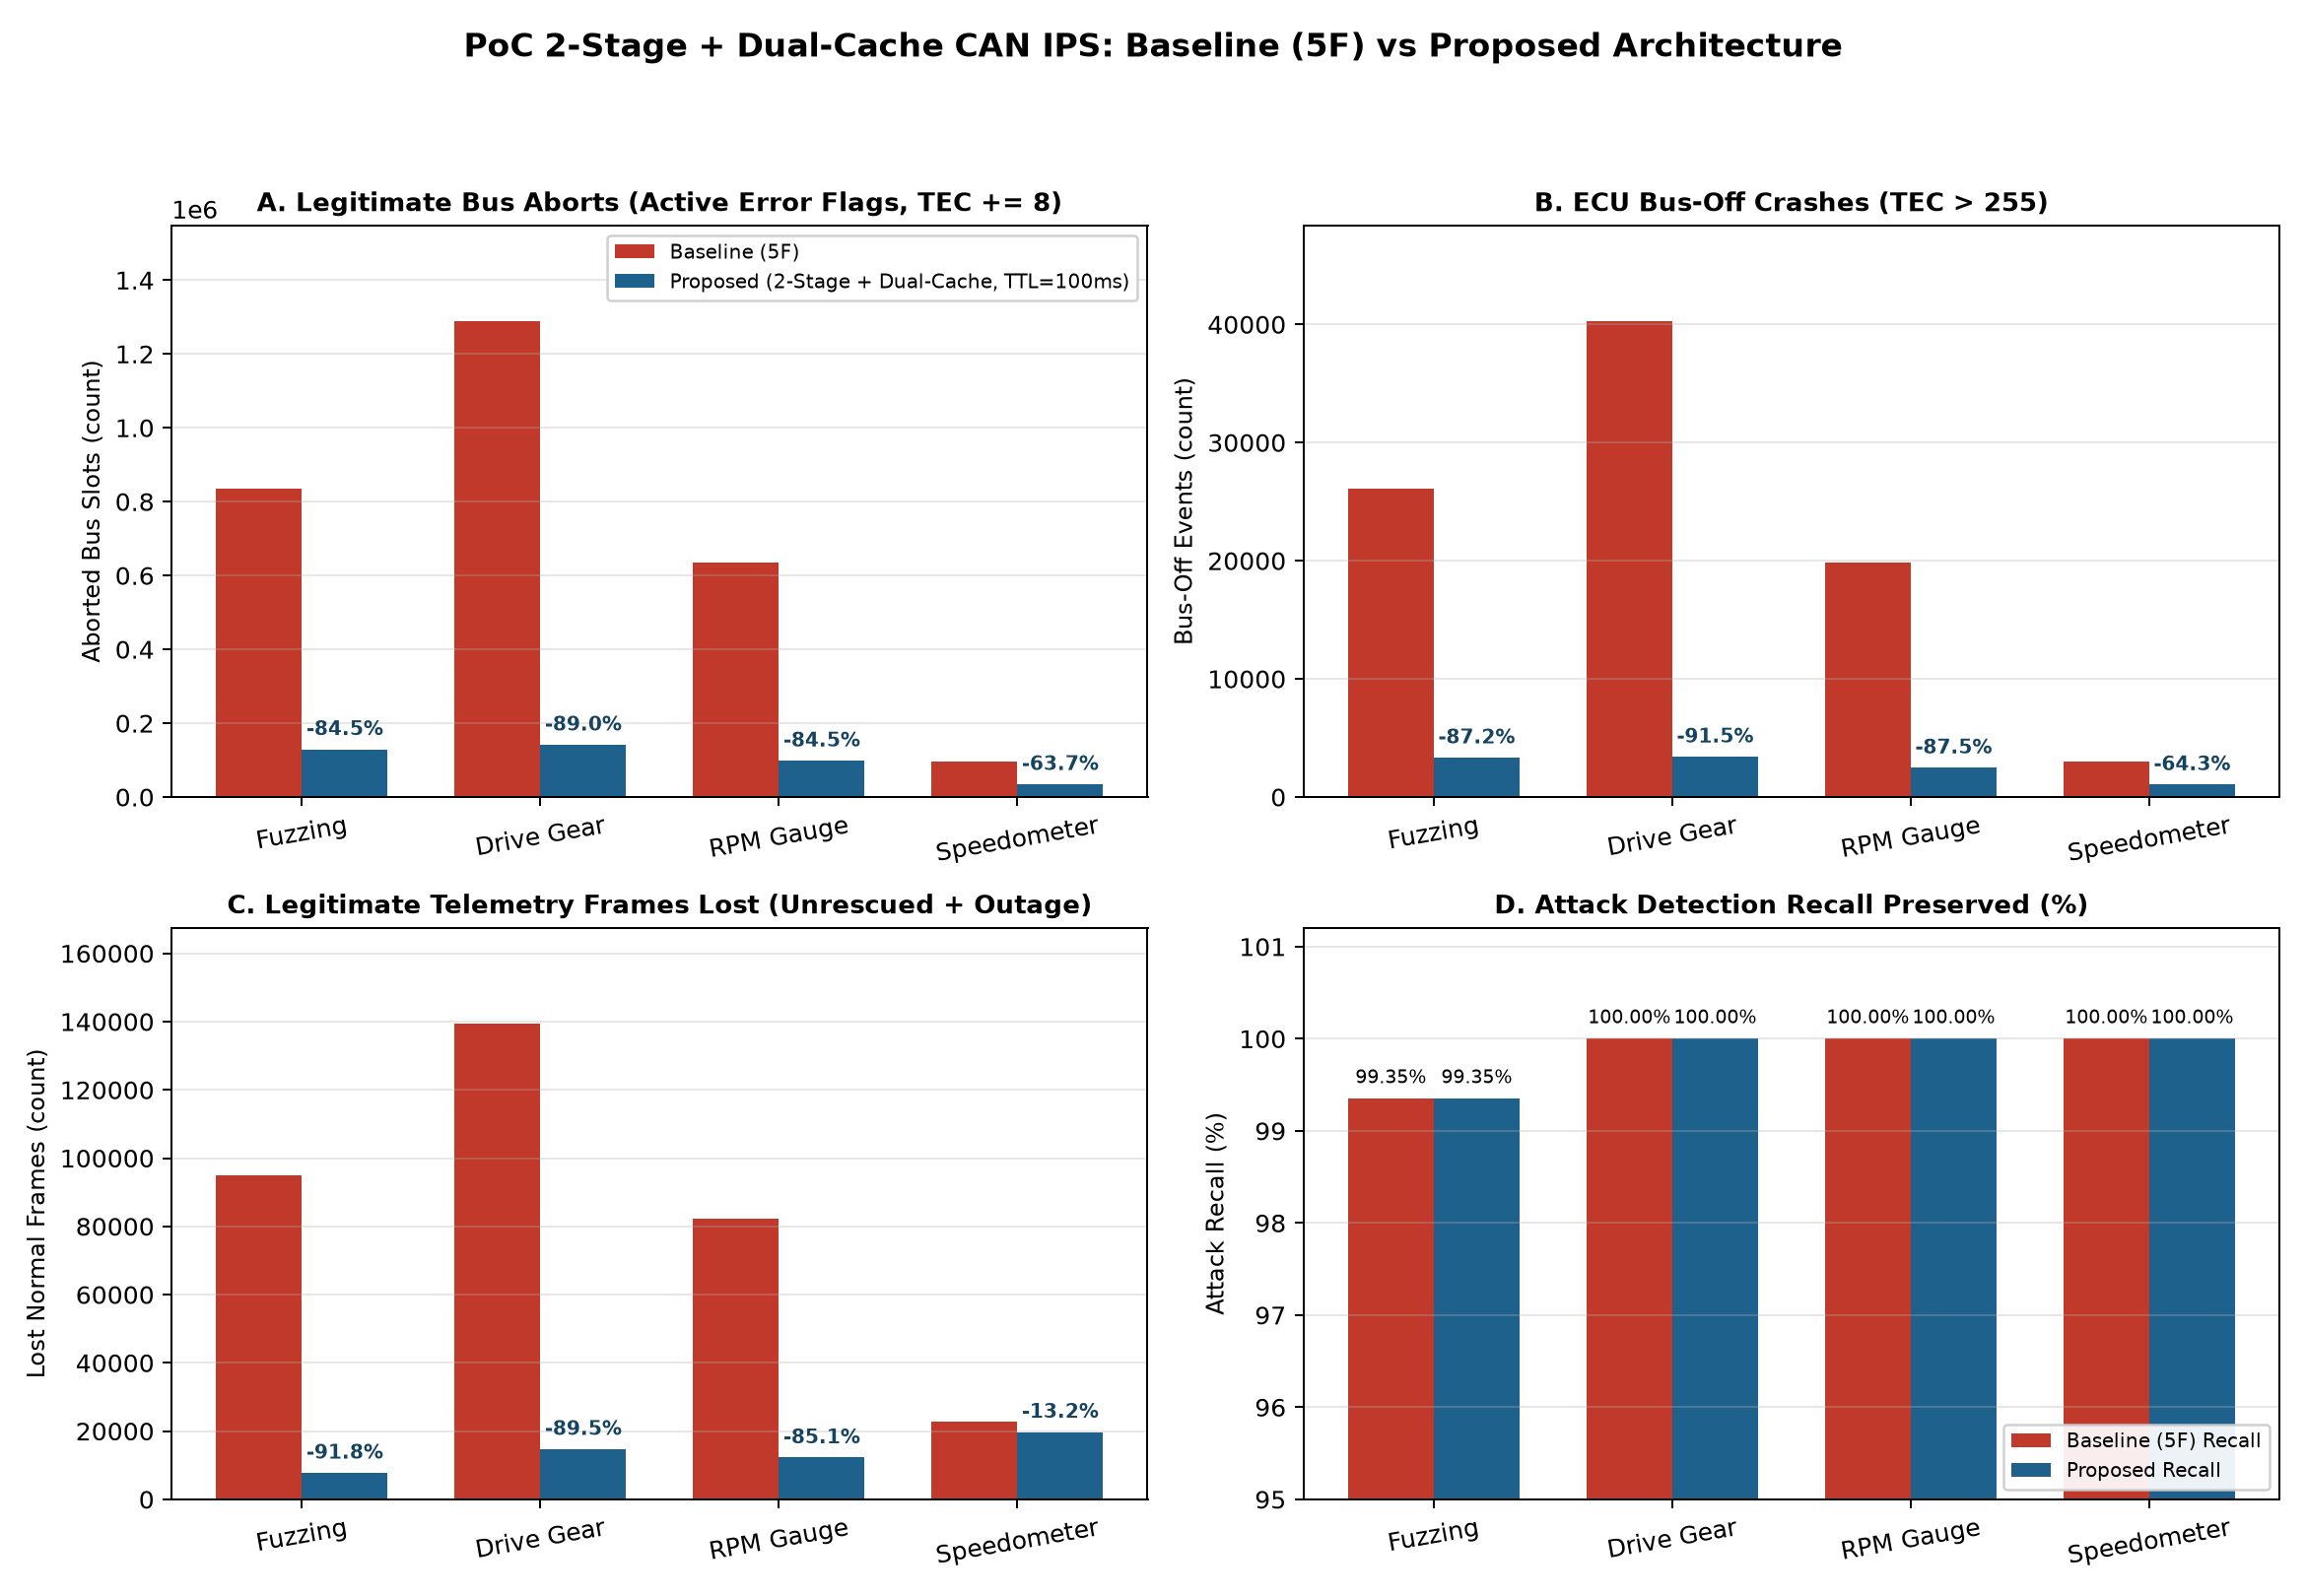
\includegraphics[width=0.90\textwidth]{fig_poc_comparison.png}
\caption{Impacto sistêmico da arquitetura Dual-Cache no simulador de confinamento de erros CAN 2.0A: (a) redução nos descartes (\textit{aborts}) de quadros legítimos, (b) queda nos eventos de \textit{Bus-Off} de ECUs, (c) redução nos quadros legítimos perdidos por falha não resgatada ou indisponibilidade e (d) preservação integral do \textit{Recall} de detecção de ataques.}
\label{fig:poc_comparison}
\end{figure*}

A análise da Tabela~\ref{tab:poc_simulation} e da Fig.~\ref{fig:poc_comparison} evidencia quatro conclusões centrais:
\begin{enumerate}
    \item \textbf{Mitigação massiva de \textit{Bus-Off} e \textit{aborts}:} Na configuração proposta (\texttt{Proposed\_DualCache\_100ms}), a arquitetura eliminou $\mathbf{64{,}34\%}$ (\textit{Speedometer}), $\mathbf{87{,}20\%}$ (\textit{Fuzzing}), $\mathbf{91{,}54\%}$ (\textit{Drive Gear}) e $\mathbf{87{,}46\%}$ (\textit{RPM Gauge}) dos desligamentos de ECUs por \textit{Bus-Off}, reduzindo transmissões legítimas abortadas entre $63{,}72\%$ e $89{,}02\%$. Consequentemente, a perda de quadros normais durante janelas de recuperação caiu em $91{,}83\%$ no \textit{Fuzzing} (de $94.979$ para $7.760$) e $89{,}45\%$ no \textit{Drive Gear} (de $139.481$ para $14.712$, reduzindo o tempo acumulado de indisponibilidade das ECUs de $2.013{,}85\text{ s}$ para $170{,}45\text{ s}$). Na simulação do protótipo em C na máquina \textit{host}, o tempo médio por inferência situou-se em $26{,}9\text{--}38{,}4~\mu\text{s}$ no Estágio 1 e $57{,}3\text{--}76{,}1~\mu\text{s}$ no Estágio 2 (sem aferição em Raspberry Pi 4 física);
    \item \textbf{Preservação integral do \textit{Recall} de ataque:} Ao contrário da cascata estática em lote no \textit{Fuzzing} (que perdia $0{,}41\%$ dos verdadeiros positivos), o fluxo temporal em tempo real preservou exatos \textbf{99,35\% de Recall} no \textit{Fuzzing} e \textbf{100,00\%} nos demais cenários. Como injeções aleatórias de \textit{Fuzzing} raramente se repetem em Cache 2, o Estágio 1 bloqueia imediatamente a primeira chegada antes de qualquer resposta tardia do Estágio 2;
    \item \textbf{Ablação do Limiar de Disparo ($k_{\text{trig}}=2$ vs. $1$):} Exigir duas detecções em Cache 1 cortou as invocações ao Estágio 2 no cenário \textit{Fuzzing} em $\mathbf{94{,}00\%}$ (de $493.727$ para $29.646$ chamadas), pois pacotes de \textit{fuzzing} únicos não geram reincidência. O custo é uma retransmissão abortada adicional antes do despacho para quadros legítimos, elevando os eventos de \textit{Bus-Off} de $3.409$ para $4.377$ no \textit{Drive Gear} e de $3.338$ para $3.602$ no \textit{Fuzzing}, constituindo um parâmetro sintonizável conforme o orçamento de CPU embarcada;
    \item \textbf{Ablação da Expiração Temporal (\textit{NoTTL} vs. $\text{TTL}=100\text{ ms}$):} Desabilitar o \textit{TTL} reduz ligeiramente os \textit{Bus-Off} (ex.: $92{,}34\%$ vs. $91{,}54\%$ no \textit{Drive Gear}). Todavia, sob ataque de \textit{Fuzzing}, o pico de entradas retidas na Cache 2 salta cerca de $\mathbf{38{,}5\times}$ — de $12.357$ para $475.720$ entradas (além de crescer de $438$ para $11.588$ no \textit{RPM Gauge} e de $1.356$ para $27.056$ no \textit{Drive Gear}). O $\text{TTL}=100\text{ ms}$ justifica-se, portanto, para limitar a ocupação de RAM e a obsolescência de vereditos, sendo explicitamente uma política de expiração de cache e não um mecanismo de detecção \textit{anti-replay}.
\end{enumerate}

\subsubsection{Análise de Sensibilidade Paramétrica do Simulador}
Para avaliar a robustez das conclusões da PoC frente à parametrização da latência do Estágio~2 ($\tau_{S2}$), da janela de recuperação de \textit{Bus-Off} ($T_{\text{rec}}$) e do $\text{TTL}$ da Cache~2, executou-se uma varredura univariada em três conjuntos representativos (\textit{Drive Gear}, \textit{Fuzzing} e \textit{Speedometer}) via \textit{flag} \mbox{\texttt{-{-}sensitivity}} de \texttt{poc\_simulator.py} (Tabela~\ref{tab:poc_sensitivity}). Três comportamentos emergem diretamente dos resultados:

\begin{itemize}
    \item \textbf{Limiar do \textit{slot} de retransmissão em $\tau_{S2}$:} Para $\tau_{S2} \in \{100\,\mu\text{s}, 200\,\mu\text{s}\}$, ambas as latências permanecem abaixo do \textit{slot} de retransmissão de $260\,\mu\text{s}$, produzindo prevenção virtualmente idêntica ($91{,}54\%$ no \textit{Drive Gear}; $87{,}19\%$ vs. $87{,}20\%$ no \textit{Fuzzing}; $64{,}31\%$ vs. $64{,}34\%$ no \textit{Speedometer}). Ao ultrapassar o \textit{slot} em $\tau_{S2} = 300\,\mu\text{s}$, ocorre um abortamento adicional enquanto o Estágio~2 ainda executa, elevando os eventos de \textit{Bus-Off} de $3.409$ para $4.379$ no \textit{Drive Gear} (e de $3.338$ para $3.603$ no \textit{Fuzzing}).
    \item \textbf{Compromisso eventos vs. telemetria perdida em $T_{\text{rec}}$:} Sob recuperação rápida compatível com contagem mínima CAN 2.0A ($T_{\text{rec}} = 3\text{ ms}$), cada ECU retorna ao barramento rapidamente, permitindo nova acumulação de erros: o total de eventos de \textit{Bus-Off} cresce ($3.409 \to 4.682$ no \textit{Drive Gear}; $1.064 \to 2.535$ no \textit{Speedometer}), mas a perda acumulada de quadros normais durante inatividade cai aproximadamente pela metade ($14.712 \to 7.282$ no \textit{Drive Gear}; $19.740 \to 10.850$ no \textit{Speedometer}). Já sob janela conservadora ($T_{\text{rec}} = 200\text{ ms}$), menos ciclos ocorrem ($2.695$ e $410$), porém a telemetria descartada sobe para $38.490$ e $23.186$ quadros, respectivamente.
    \item \textbf{Estabilidade do $\text{TTL}$ e invariância de \textit{Recall}:} Variar o $\text{TTL}$ entre $20\text{ ms}$ e $500\text{ ms}$ mantém a prevenção de \textit{Bus-Off} estável em todos os cenários ($91{,}34\%\text{--}91{,}78\%$ no \textit{Drive Gear}; $86{,}75\%\text{--}87{,}48\%$ no \textit{Fuzzing}; $64{,}04\%\text{--}64{,}85\%$ no \textit{Speedometer}), confirmando que $\text{TTL}=100\text{ ms}$ equilibra redução de re-invocações do Estágio~2 frente a $20\text{ ms}$ ($66.810$ vs. $107.389$ no \textit{Drive Gear}) sem reter estados antigos como $500\text{ ms}$. Em todas as $18$ execuções da varredura, o \textit{Attack Recall} permaneceu rigorosamente inalterado ($100{,}00\%$ no \textit{Drive Gear} e \textit{Speedometer}; $99{,}35\%$ no \textit{Fuzzing}).
\end{itemize}

\begin{table*}[t]
\centering
\caption{Análise de sensibilidade paramétrica do simulador da PoC ($24$ execuções em \texttt{poc\_sensitivity\_results.csv}). Valores de Prev. (\%) referem-se à redução relativa de Bus-Off frente ao \texttt{Baseline\_5F} de cada conjunto (Drive Gear: $40.277$ Bus-Off / $139.481$ normais perdidos; Fuzzing: $26.076$ / $94.979$; Speedometer: $2.984$ / $22.736$).}
\label{tab:poc_sensitivity}
\scriptsize
\setlength{\tabcolsep}{4pt}
\renewcommand{\arraystretch}{1.12}
\begin{tabular}{@{}llcccccc@{}}
\toprule
\textbf{Dataset} & \textbf{Configuração} & \textbf{Parâmetros ($\tau_{S2}$ / $T_{\text{rec}}$ / TTL)} & \textbf{Bus-Off} & \textbf{Prev. (\%)} & \textbf{Norm. Perd.} & \textbf{Invoc. E2} & \textbf{Rec. At.} \\
\midrule
\textit{Drive Gear} & \texttt{Sens\_S2Lat\_100us} & $100\,\mu\text{s}$ / $50\text{ ms}$ / $100\text{ ms}$ & $3.409$ & $91{,}54\%$ & $14.712$ & $66.843$ & $100{,}00\%$ \\
\textit{Drive Gear} & \texttt{Proposed\_DualCache\_100ms} (Ref.) & $200\,\mu\text{s}$ / $50\text{ ms}$ / $100\text{ ms}$ & $3.409$ & $91{,}54\%$ & $14.712$ & $66.810$ & $100{,}00\%$ \\
\textit{Drive Gear} & \texttt{Sens\_S2Lat\_300us} & $300\,\mu\text{s}$ / $50\text{ ms}$ / $100\text{ ms}$ & $4.379$ & $89{,}13\%$ & $17.842$ & $104.910$ & $100{,}00\%$ \\
\textit{Drive Gear} & \texttt{Sens\_Rec\_3ms} & $200\,\mu\text{s}$ / $3\text{ ms}$ / $100\text{ ms}$ & $4.682$ & $88{,}38\%$ & $7.282$ & $68.769$ & $100{,}00\%$ \\
\textit{Drive Gear} & \texttt{Sens\_Rec\_200ms} & $200\,\mu\text{s}$ / $200\text{ ms}$ / $100\text{ ms}$ & $2.695$ & $93{,}31\%$ & $38.490$ & $62.773$ & $100{,}00\%$ \\
\textit{Drive Gear} & \texttt{Sens\_TTL\_20ms} & $200\,\mu\text{s}$ / $50\text{ ms}$ / $20\text{ ms}$ & $3.488$ & $91{,}34\%$ & $15.071$ & $107.389$ & $100{,}00\%$ \\
\textit{Drive Gear} & \texttt{Sens\_TTL\_500ms} & $200\,\mu\text{s}$ / $50\text{ ms}$ / $500\text{ ms}$ & $3.312$ & $91{,}78\%$ & $14.272$ & $51.548$ & $100{,}00\%$ \\
\midrule
\textit{Fuzzing} & \texttt{Sens\_S2Lat\_100us} & $100\,\mu\text{s}$ / $50\text{ ms}$ / $100\text{ ms}$ & $3.340$ & $87{,}19\%$ & $7.759$ & $493.773$ & $99{,}35\%$ \\
\textit{Fuzzing} & \texttt{Proposed\_DualCache\_100ms} (Ref.) & $200\,\mu\text{s}$ / $50\text{ ms}$ / $100\text{ ms}$ & $3.338$ & $87{,}20\%$ & $7.760$ & $493.727$ & $99{,}35\%$ \\
\textit{Fuzzing} & \texttt{Sens\_S2Lat\_300us} & $300\,\mu\text{s}$ / $50\text{ ms}$ / $100\text{ ms}$ & $3.603$ & $86{,}18\%$ & $8.516$ & $500.561$ & $99{,}35\%$ \\
\textit{Fuzzing} & \texttt{Sens\_Rec\_3ms} & $200\,\mu\text{s}$ / $3\text{ ms}$ / $100\text{ ms}$ & $4.212$ & $83{,}85\%$ & $5.601$ & $494.395$ & $99{,}35\%$ \\
\textit{Fuzzing} & \texttt{Sens\_Rec\_200ms} & $200\,\mu\text{s}$ / $200\text{ ms}$ / $100\text{ ms}$ & $2.887$ & $88{,}93\%$ & $14.951$ & $492.591$ & $99{,}35\%$ \\
\textit{Fuzzing} & \texttt{Sens\_TTL\_20ms} & $200\,\mu\text{s}$ / $50\text{ ms}$ / $20\text{ ms}$ & $3.454$ & $86{,}75\%$ & $8.195$ & $499.732$ & $99{,}35\%$ \\
\textit{Fuzzing} & \texttt{Sens\_TTL\_500ms} & $200\,\mu\text{s}$ / $50\text{ ms}$ / $500\text{ ms}$ & $3.266$ & $87{,}48\%$ & $7.556$ & $487.879$ & $99{,}35\%$ \\
\midrule
\textit{Speedometer} & \texttt{Sens\_S2Lat\_100us} & $100\,\mu\text{s}$ / $50\text{ ms}$ / $100\text{ ms}$ & $1.065$ & $64{,}31\%$ & $19.741$ & $3.136$ & $100{,}00\%$ \\
\textit{Speedometer} & \texttt{Proposed\_DualCache\_100ms} (Ref.) & $200\,\mu\text{s}$ / $50\text{ ms}$ / $100\text{ ms}$ & $1.064$ & $64{,}34\%$ & $19.740$ & $3.132$ & $100{,}00\%$ \\
\textit{Speedometer} & \texttt{Sens\_S2Lat\_300us} & $300\,\mu\text{s}$ / $50\text{ ms}$ / $100\text{ ms}$ & $1.111$ & $62{,}77\%$ & $19.779$ & $4.439$ & $100{,}00\%$ \\
\textit{Speedometer} & \texttt{Sens\_Rec\_3ms} & $200\,\mu\text{s}$ / $3\text{ ms}$ / $100\text{ ms}$ & $2.535$ & $15{,}05\%$ & $10.850$ & $4.592$ & $100{,}00\%$ \\
\textit{Speedometer} & \texttt{Sens\_Rec\_200ms} & $200\,\mu\text{s}$ / $200\text{ ms}$ / $100\text{ ms}$ & $410$ & $86{,}26\%$ & $23.186$ & $2.331$ & $100{,}00\%$ \\
\textit{Speedometer} & \texttt{Sens\_TTL\_20ms} & $200\,\mu\text{s}$ / $50\text{ ms}$ / $20\text{ ms}$ & $1.073$ & $64{,}04\%$ & $19.746$ & $3.903$ & $100{,}00\%$ \\
\textit{Speedometer} & \texttt{Sens\_TTL\_500ms} & $200\,\mu\text{s}$ / $50\text{ ms}$ / $500\text{ ms}$ & $1.049$ & $64{,}85\%$ & $19.729$ & $2.343$ & $100{,}00\%$ \\
\bottomrule
\end{tabular}
\end{table*}

\section{Conclusão, Limitações e Trabalhos Futuros}

Este trabalho realizou a replicação completa e a validação estatística do Sistema de Prevenção de Intrusão (IPS) para redes CAN automotivas proposto por Araujo-Filho \textit{et al.} \cite{araujo2021efficient}, estendendo-o para um segundo conjunto de dados independente (\textit{Prototype Speedometer Spoofing}) e propondo uma arquitetura IPS em dois estágios com \textit{Dual-Cache} validada em prova de conceito. A replicação confirmou que o algoritmo não supervisionado \textit{Isolation Forest} operando sobre apenas os primeiros bytes do campo de dados atinge acurácias entre $98{,}32\%$ e $99{,}14\%$ com $\text{iForest\_5F}$ (e até $99{,}58\%$ com 8 bytes) nos ataques do \textit{Car-Hacking}, bem como $99{,}12\%$ de acurácia e $100{,}00\%$ de \textit{Recall} com $\text{iForest\_3F}$ no \textit{Speedometer Spoofing}. Investigamos também o papel determinante da profundidade (\texttt{max\_samples}) para isolar anomalias conjuntas e o efeito de diluição causado por bytes finais redundantes (\texttt{0x00}).

A partir do diagnóstico das limitações do sistema de referência, analisamos quatro aspectos estruturais:
\begin{enumerate}
    \item \textbf{Ausência do Identificador (\textit{CAN ID}) (Mitigada no Estágio 2):} Na arquitetura original, o modelo recebe apenas $[D_0, \dots, D_{N-1}]$, modelando a união de todos os IDs e gerando colisões inter-mensagens. A extensão proposta em Estágio 2 ($\text{CAN\_ID} + 8\text{ bytes}$) com roteamento híbrido por identificador ($\text{iForest\_Hybrid\_Fallback}$) atacou diretamente essa lacuna, resgatando de $53{,}42\%$ a $92{,}37\%$ dos falsos positivos em cascata;
    \item \textbf{Impacto de Falsos Positivos e Risco de \textit{Bus-Off} (Mitigado pelo \textit{Dual-Cache}):} Falsos positivos consecutivos de \textit{Error Frames} ($\text{TEC} \mathrel{+}= 8$) levariam ECUs legítimas ao estado de \textit{Bus-Off} após $32$ aborts. O protótipo em três \textit{threads} com \textit{Dual-Cache} e $\text{TTL}=100\text{ ms}$ eliminou $64{,}34\%$ a $91{,}54\%$ dos desligamentos estimados por \textit{CAN ID} no modelo orientado a traços sem perda de \textit{Recall}, mantendo consumo de memória limitado;
    \item \textbf{Cegueira à dinâmica temporal ($\Delta t$) e ataques de inundação (DoS/Replay):} Ambos os estágios avaliam quadros de modo estritamente independente (\textit{stateless}); a Cache 2 limita apenas a memória e a permanência do veredicto em cache ($\text{TTL}=100\text{ ms}$), sem oferecer proteção \textit{anti-replay}. Consequentemente, ataques DoS ou de \textit{Replay} reproduzindo payloads legítimos permanecem invisíveis sem a inclusão explícita do intervalo inter-chegadas $\Delta t$ por identificador;
    \item \textbf{Sensibilidade ao hiperparâmetro \texttt{contamination} sob validação balanceada:} Como os \textit{folds} possuem razão 50\% normal e 50\% ataque (diferente do tráfego real $\sim 86\%$ normal), a calibragem tende a manter falsos positivos residuais não desprezíveis, como observado no cenário \textit{Speedometer} (em que restaram $2.501$ FPs após o Estágio 2).
\end{enumerate}

Como trabalhos futuros, em decorrência das restrições de cronograma deste projeto que impediram a execução física na placa alvo, planejamos: (i) implantar e aferir as latências reais de ponta a ponta do protótipo em três \textit{threads} na plataforma Raspberry Pi 4 sob barramento CAN físico; (ii) incorporar atributos temporais ($\Delta t$) nos modelos para detecção conjunta de \textit{DoS} e \textit{Replay}; e (iii) realizar o levantamento bibliográfico de outros estudos sobre o conjunto de dados \textit{Prototype} para compor uma análise comparativa externa.

\IEEEtriggeratref{6}
\begin{thebibliography}{00}

\bibitem{araujo2021efficient}
P. F. de Araujo-Filho, A. J. Pinheiro, G. Kaddoum, D. R. Campelo, and F. L. Soares, ``An efficient intrusion prevention system for CAN: Hindering cyber-attacks with a low-cost platform,'' \textit{IEEE Access}, vol. 9, pp. 166855--166869, 2021.

\bibitem{bosch1991can}
Robert Bosch GmbH, \textit{CAN Specification Version 2.0}. Stuttgart, Germany: Bosch, 1991.

\bibitem{koscher2010experimental}
K. Koscher \textit{et al.}, ``Experimental security analysis of a modern automobile,'' in \textit{Proc. IEEE Symp. Security and Privacy (SP)}, Oakland, CA, USA, 2010, pp. 447--462.

\bibitem{checkoway2011comprehensive}
S. Checkoway \textit{et al.}, ``Comprehensive experimental analyses of automotive attack surfaces,'' in \textit{Proc. 20th USENIX Security Symp.}, San Francisco, CA, USA, 2011, pp. 77--92.

\bibitem{miller2015remote}
C. Miller and C. Valasek, ``Remote exploitation of an unaltered passenger vehicle,'' \textit{Black Hat USA}, vol. 2015, p. 91, 2015.

\bibitem{seo2018gids}
E. Seo, H. M. Song, and H. K. Kim, ``GIDS: GAN based intrusion detection system for in-vehicle network,'' in \textit{Proc. 16th Annu. Conf. Privacy, Security and Trust (PST)}, Belfast, Ireland, 2018, pp. 1--6.

\bibitem{song2020invehicle}
H. M. Song, J. Woo, and H. K. Kim, ``In-vehicle network intrusion detection using deep convolutional neural network,'' \textit{Vehicular Communications}, vol. 21, p. 100198, Jan. 2020.

\bibitem{yang2021mth}
L. Yang, A. Moubayed, and A. Shami, ``MTH-IDS: A multitiered hybrid intrusion detection system for Internet of Vehicles,'' \textit{IEEE Internet of Things Journal}, vol. 9, no. 1, pp. 616--632, Jan. 2022.

\bibitem{liu2008isolation}
F. T. Liu, K. M. Ting, and Z.-H. Zhou, ``Isolation forest,'' in \textit{Proc. 8th IEEE Int. Conf. Data Mining (ICDM)}, Pisa, Italy, 2008, pp. 413--422.

\bibitem{scholkopf2001estimating}
B. Sch{\"o}lkopf, J. C. Platt, J. Shawe-Taylor, A. J. Smola, and R. C. Williamson, ``Estimating the support of a high-dimensional distribution,'' \textit{Neural Computation}, vol. 13, no. 7, pp. 1443--1471, Jul. 2001.

\bibitem{wang2018hardware}
Q. Wang and S. Sawhney, ``VeCure: A practical security framework to protect the CAN bus of vehicles,'' in \textit{Proc. Int. Conf. Internet of Things (IOT)}, Cambridge, MA, USA, 2014, pp. 13--18.

\bibitem{kvaser_error}
Kvaser AB, ``CAN Protocol Tutorial: Error Handling,'' \textit{Kvaser CAN Learning}. [Online]. Available: \url{https://kvaser.com/lesson/can-error-handling/}

\bibitem{fourtu_can_dataset}
``Automotive CAN bus intrusion dataset,'' \textit{4TU.ResearchData}, Dataset, DOI: \url{10.4121/uuid:b74b4928-c377-4585-9432-2004dfa20a5d}. [Online]. Available: \url{https://data.4tu.nl/articles/_/12696950/2}

\end{thebibliography}

\end{document}
